A fit to the \mll distribution is performed in search of the characteristic edge signature described in section~\ref{sec:somesignalsection}. Different functions are used to model the contributions of the potential signal, flavour-symmetric backgrounds, and backgrounds containing a Z boson. To fully exploit the available information, an unbinned maximum-likelihood fit is performed simultaneously to the \EE, \MM, and \EM event samples for both the signal and forward dilepton selection in the signal region.

\section{Background and signal models}



\subsection{Model for Z backgrounds}
\label{sec:Zmodel}
The background model for events containing a Z boson contains of two components: one model for the Z boson peak and one for the contribution of the Drell--Yan continuum. The latter one is a simple falling exponential. The peak model consists of a Breit-Wigner function with mean and widths fixed to the DPG values for the Z boson, convolved with a double-sided crystal ball function~\cite{Crystal}. The first component models the physical peak while the latter accounts for the detector resolution and radiative corrections to the Z lineshape. The double-sided crystal ball itself consists of a Gaussian core and exponential falloffs to both sides of the peak, parametrized as
\begin{eqnarray*}
\mathcal{P}_{DSCB}(m_{\ell\ell}) = \begin{cases} A_{1} (B_{1}-\frac{m_{ll}-\mu_{CB}}{\sigma_{CB}})^{-n_{1}} &\mbox{if } \frac{m_{ll}-\mu_{CB}}{\sigma_{CB}}<-\alpha_{1} \\
\textrm{exp}\left(-\frac{(m_{ll}-\mu_{CB})^2}{2\sigma_{CB}^2}\right) &\mbox{if } -\alpha_{1}<\frac{m_{ll}-\mu_{CB}}{\sigma_{CB}}<\alpha_{2} \\
A_{2} (B_{2}+\frac{m_{ll}-\mu_{CB}}{\sigma_{CB}})^{-n_{2}} &\mbox{if } \frac{m_{ll}-\mu_{CB}}{\sigma_{CB}}>\alpha_{2} \\
\end{cases}
\end{eqnarray*}
where $\sigma_{CB}$ and $\mu_{CB}$ are the parameters of the central Gaussian and the $n_i$ and $\alpha_i$ govern the transition to and the shape of the exponential falloff. The $A_i$ and $B_i$ are substitutions for
\begin{eqnarray*}
A_{i} = \left(\frac{n_{i}}{|\alpha_{i}|}\right)^{n_{i}} \cdot \textrm{exp}\left(-\frac{|\alpha_{i}|^2}{2}\right) \quad \textrm{and}\quad B_{i} = \frac{n_{i}}{|\alpha_{i}|}-|\alpha_{i}| .
\end{eqnarray*}
Taking into account also the exponential function described the Drell--Yan continuum, the full description is therefore 
\begin{eqnarray*}
\mathcal{P}_{DY} (m_{\ell\ell}) = f_{exp}\mathcal{P}_{exp}(m_{\ell\ell})+(1-f_{exp})\int \mathcal{P}_{DSCB}(m_{\ell\ell})\mathcal{P}_{BW}(m_{\ell\ell}-m') dm',
\end{eqnarray*}
where $f_{exp}$ is the fraction that the exponential component contributes to the full PDF. 

This model is fitted to the data in the Drell--Yan control region separately for \EE and \MM events after flavour-symmetric backgrounds are subtracted using OF events. Afterwards, all parameters of the model are fixed and only the normalization is left floating in the fit in the signal region. The resulting fits are shown in Figure~\ref{fig:dyFits} and are a good description of the distribution in all cases. 

\begin{figure}[htbp]
\centering
\begin{minipage}[t]{0.49\textwidth}
  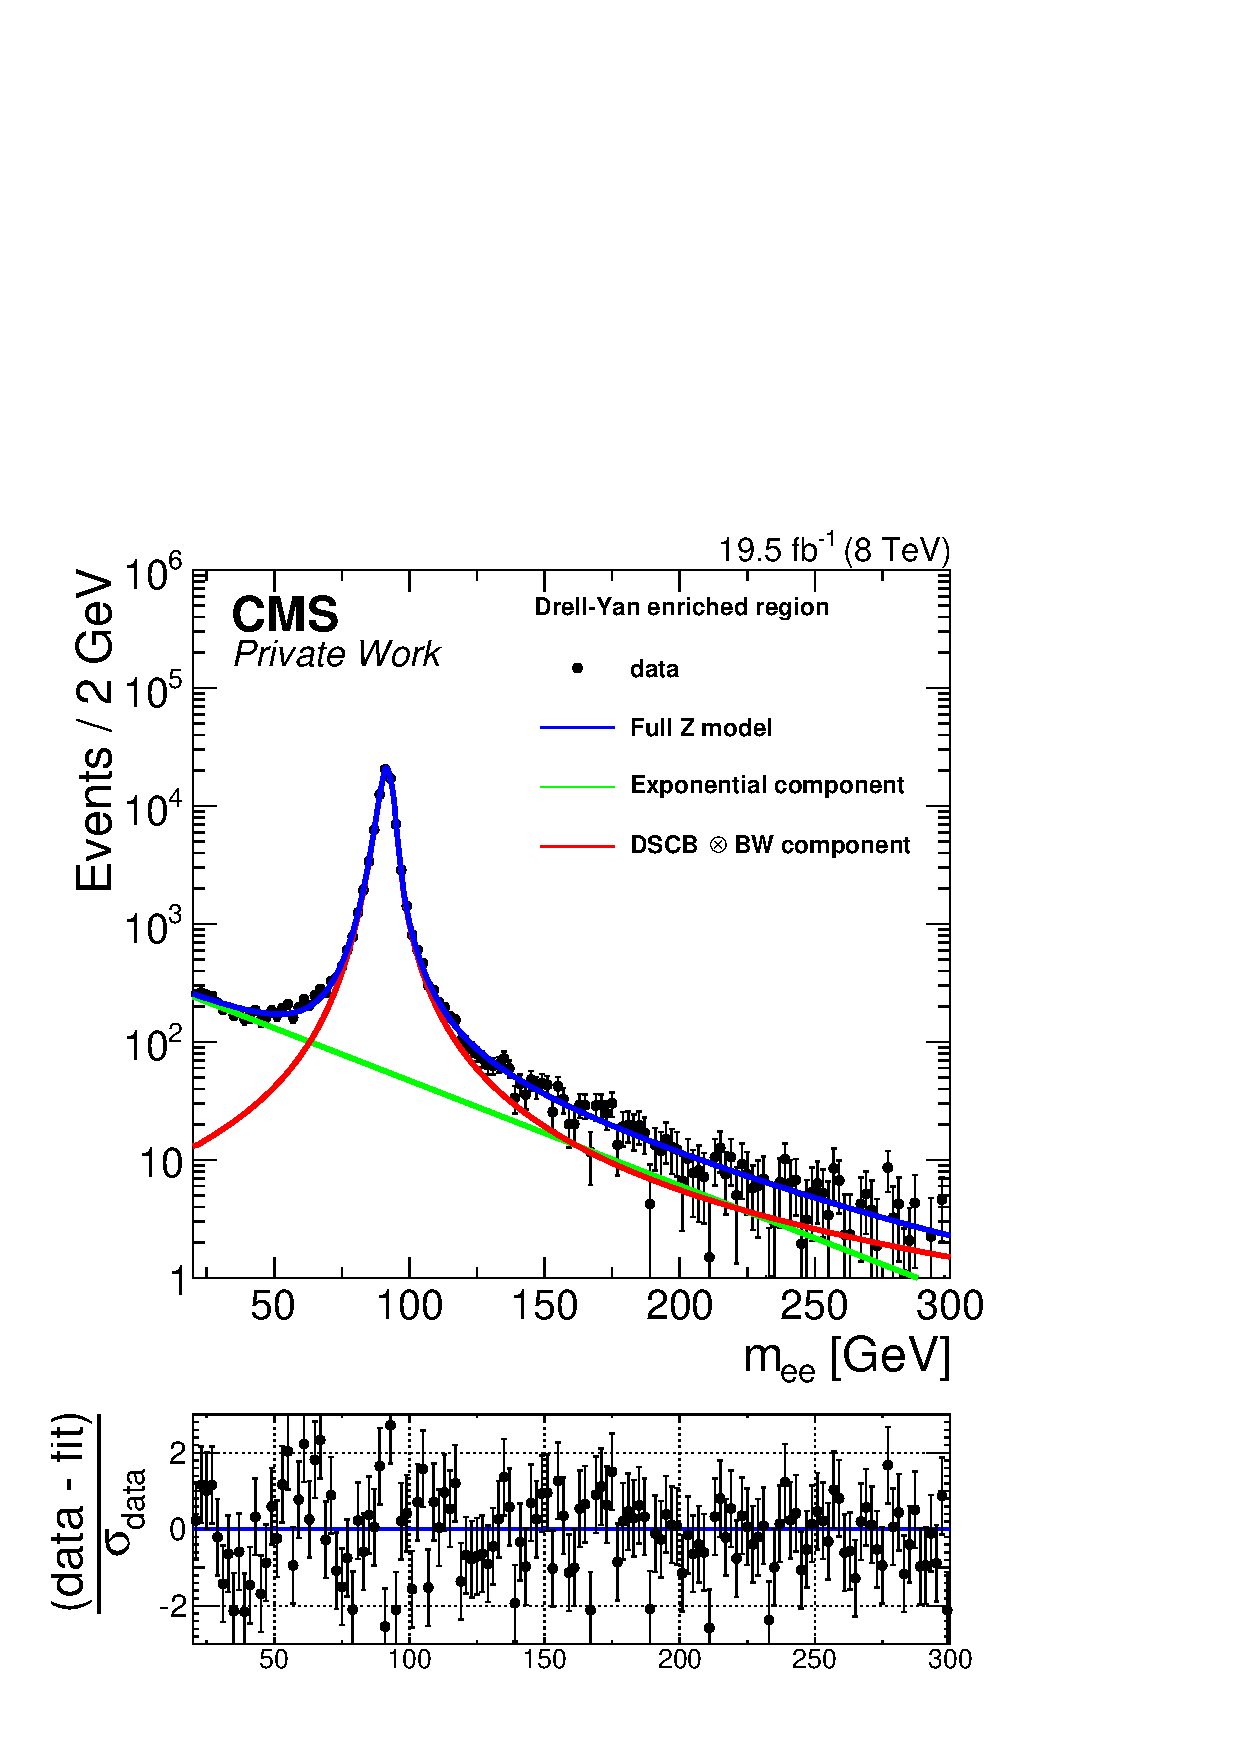
\includegraphics[width=\textwidth]{plots/results/fit/expoFitEE_Log_Central.pdf}
\end{minipage}
\begin{minipage}[t]{0.49\textwidth}
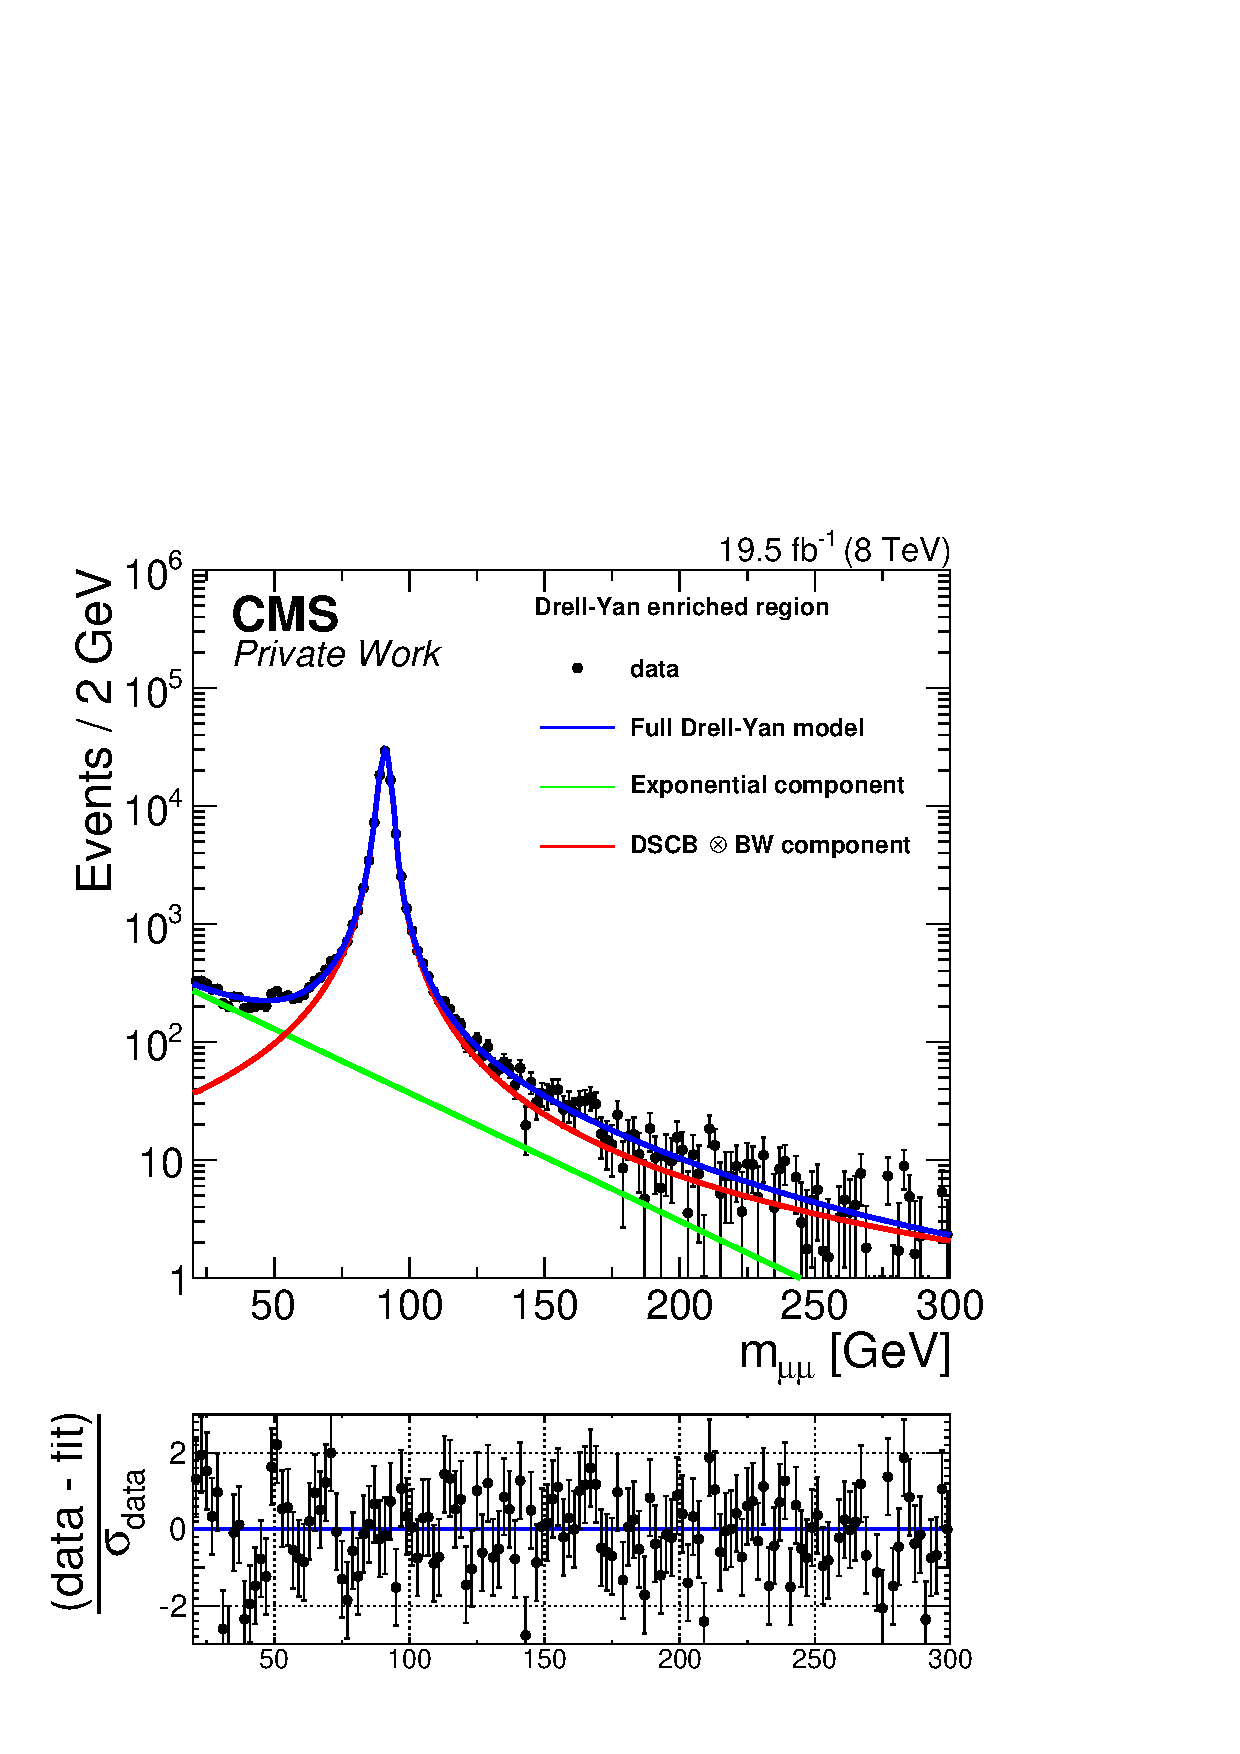
\includegraphics[width=\textwidth]{plots/results/fit/expoFitMM_Log_Central.pdf}
\end{minipage}
\begin{minipage}[t]{0.49\textwidth}
  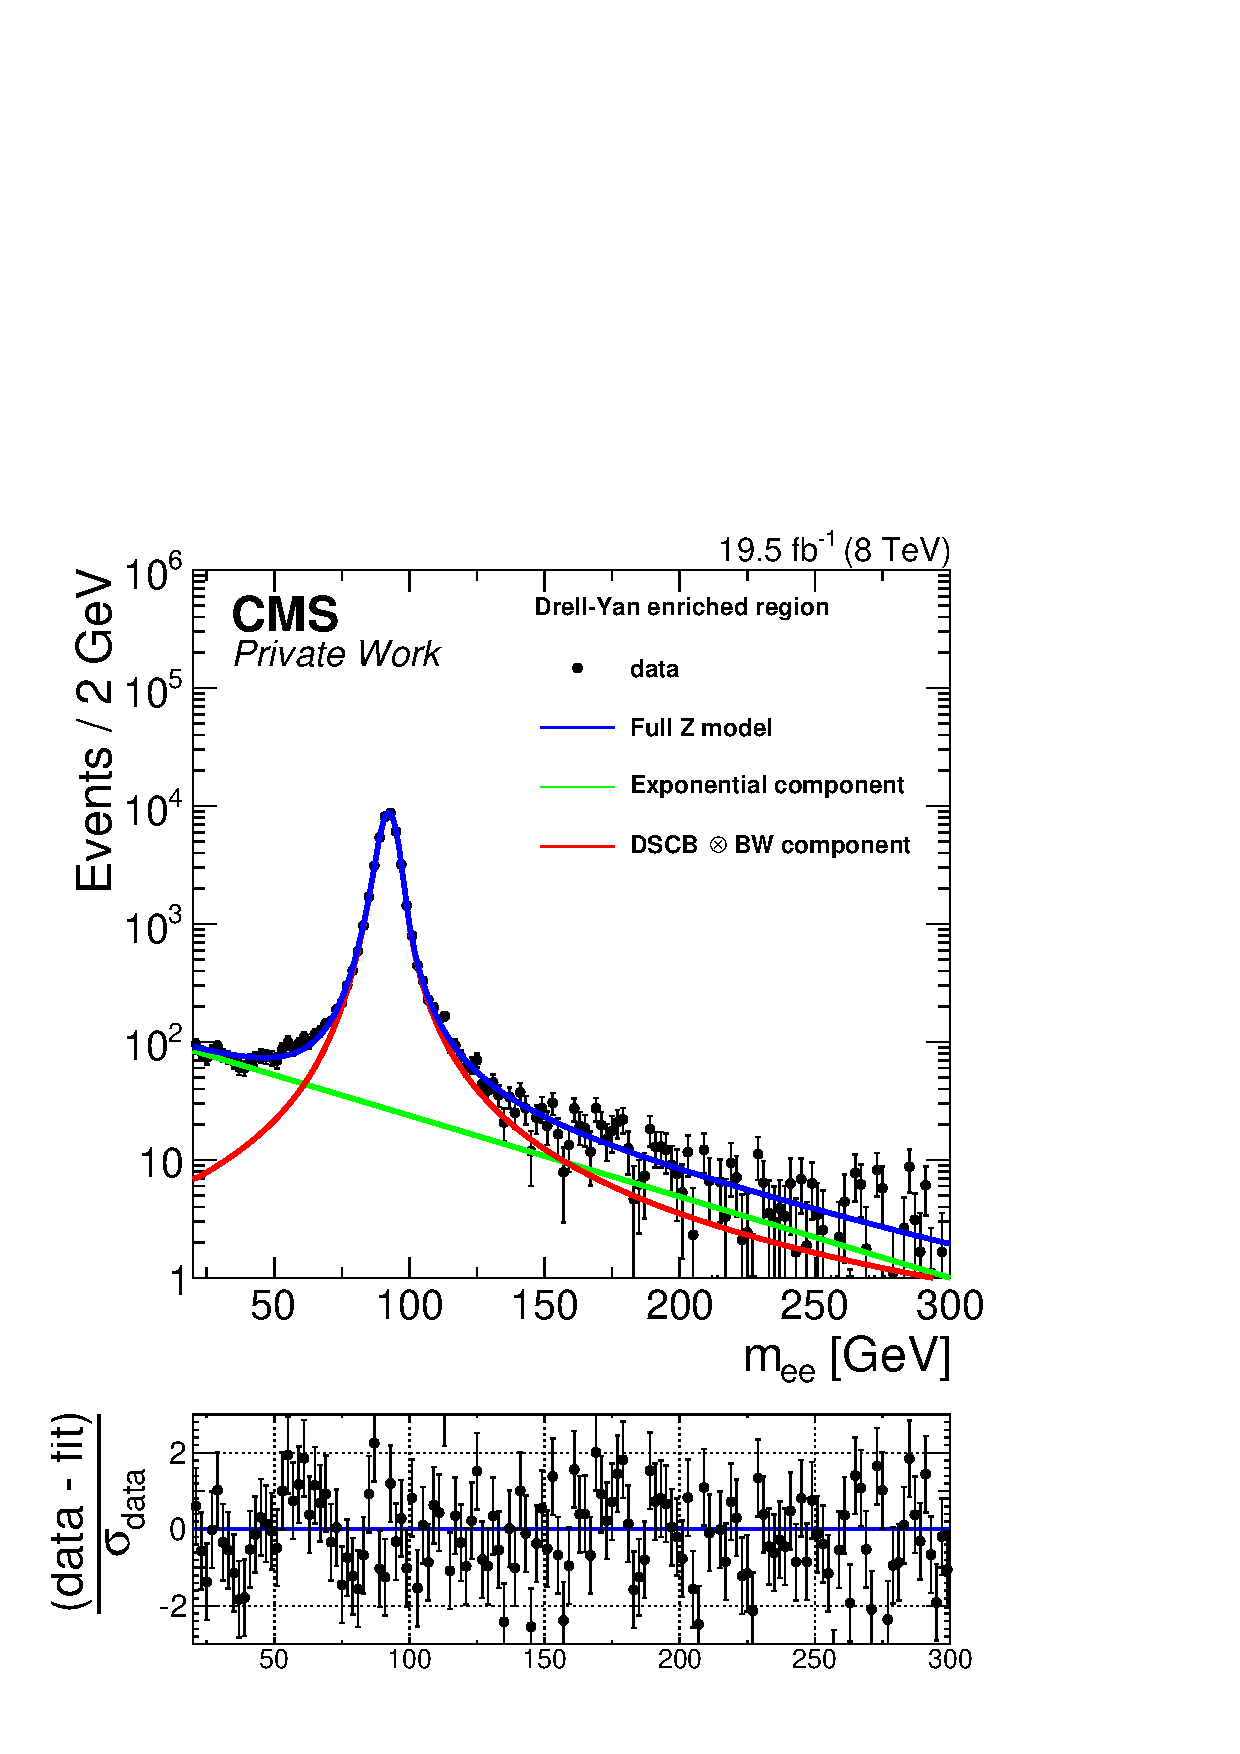
\includegraphics[width=\textwidth]{plots/results/fit/expoFitEE_Log_Forward.pdf}
\end{minipage}
\begin{minipage}[t]{0.49\textwidth}
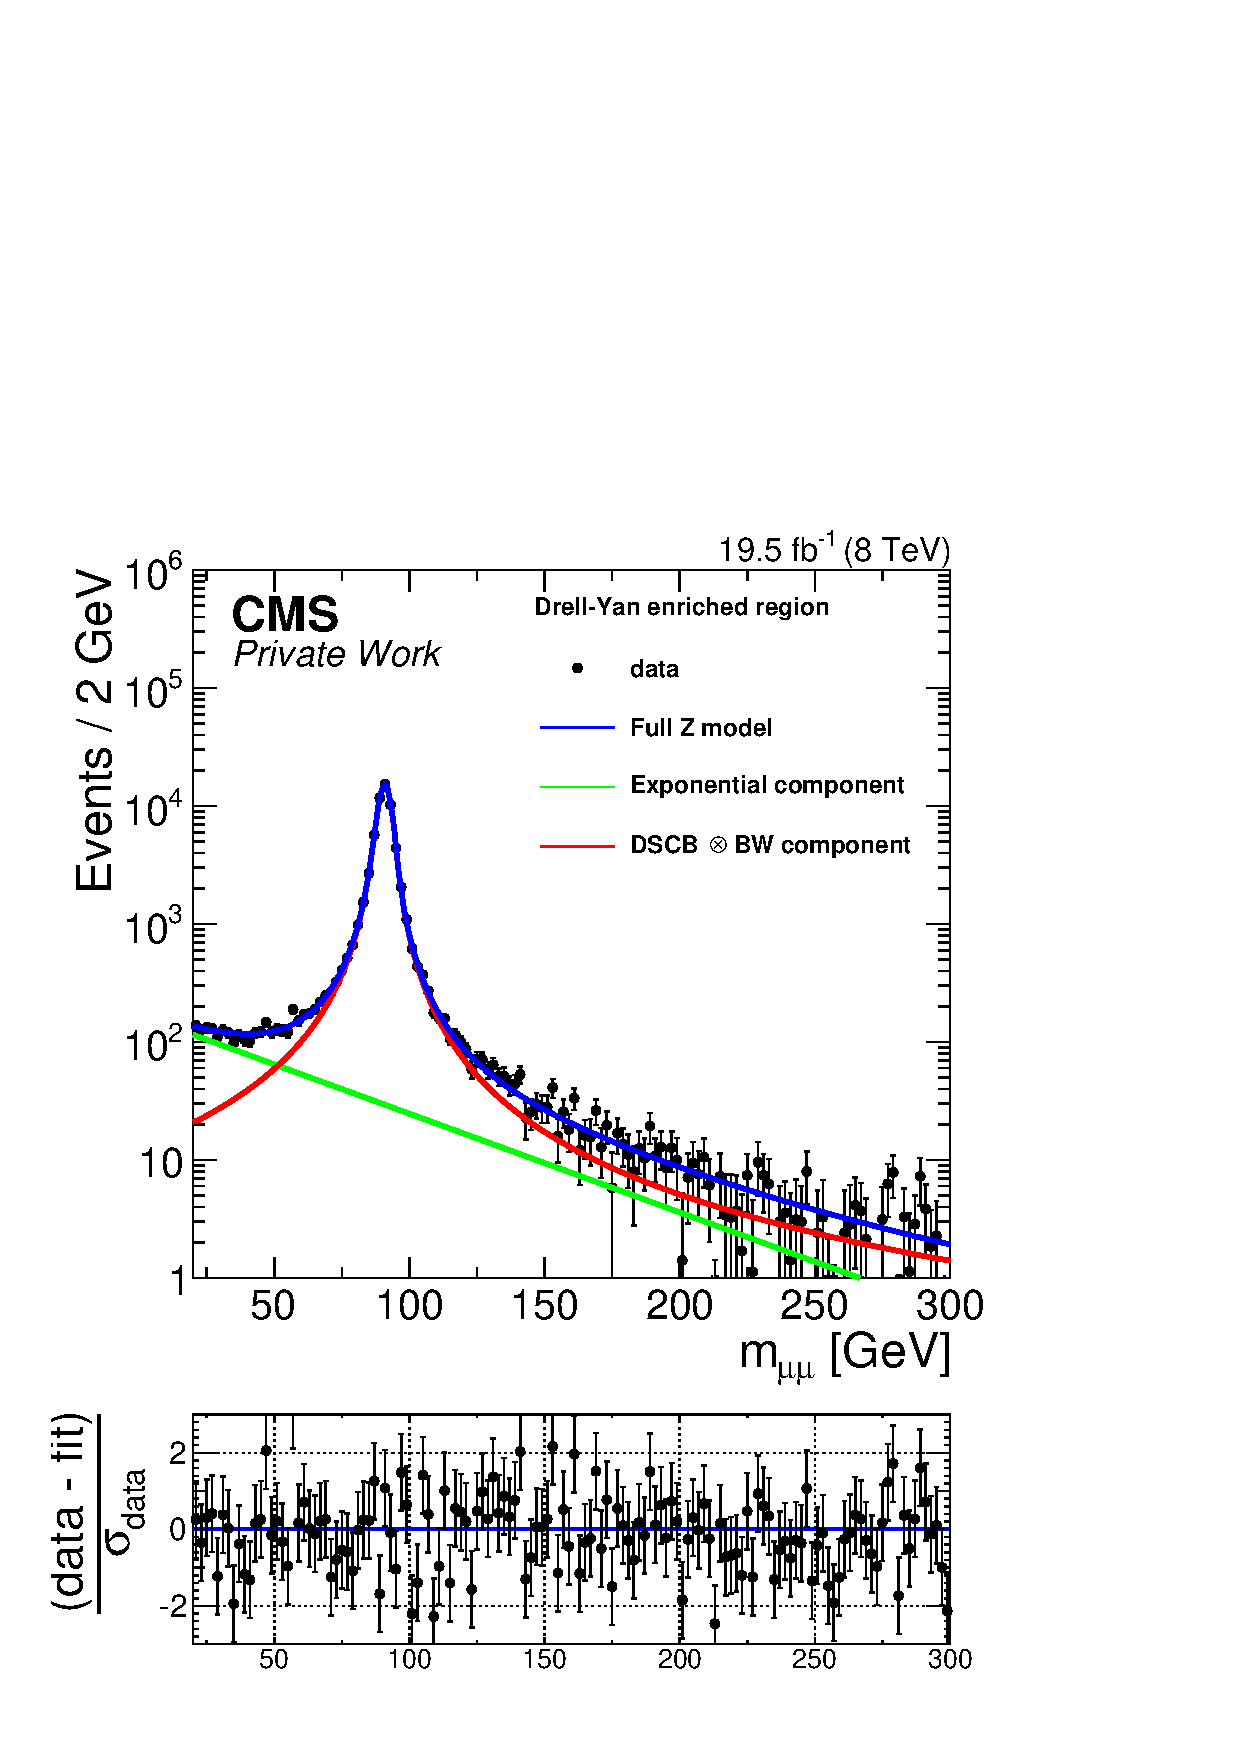
\includegraphics[width=\textwidth]{plots/results/fit/expoFitMM_Log_Forward.pdf}
\end{minipage}
\caption{Fit to the \mll distribution in the Drell--Yan control region separately for \EE (left) and \MM (right) events in the central (top) and forward (bottom) dilepton selection. The data is shown as black points while the resulting fit is shown in blue. The red and green lines show the contributions of the continuum model and the peak model to the combined fit.}
\label{fig:dyFits}
\end{figure}


\subsection{Model for flavour-symmetric backgrounds}

\subsubsection{Nominal parametrization}
Flavour-symmetric models are described with a model consisting of three parts. The rising flank of the distribution is modelled with a power law, the peak region with a fourth order polynomial and the falling flank with an exponential falloff. 

\begin{eqnarray*}
{\mathcal{P}}_{FS}(m_{\ell\ell}) = \begin{cases} {\mathcal{P}}_{FSE,1}(m_{\ell\ell}) = c_{1} \cdot m_{\ell\ell}^{\alpha} &\mbox{if } 20\GeV < m_{\ell\ell} < m_{\ell\ell}^{(1)} \\
{\mathcal{P}}_{FS,2}(m_{\ell\ell}) = \sum_{i=0}^{3} c_{2,i} \cdot m_{\ell\ell}^{i} & \mbox{if } m_{\ell\ell}^{(1)}<m_{\ell\ell}<m_{\ell\ell}^{(2)} \\
{\mathcal{P}}_{FS,3}(m_{\ell\ell}) = c_{3}\cdot e^{-\beta m_{\ell\ell}} & \mbox{if } m_{\ell\ell}^{(2)}<m_{\ell\ell}<300\GeV \\
\end{cases} 
\end{eqnarray*}
where $m_{\ell\ell}^{(1)}$ and $m_{\ell\ell}^{(2)}$ are the transition points between the different parts of the model. The model is required to be normalized and also to be continuously differentiable in $m_{\ell\ell}^{(1)}$ and $m_{\ell\ell}^{(2)}$, reducing the number of free parameters to five: $\mathbf{p}_{FS} = (m_{\ell\ell}^{(1)},m_{\ell\ell}^{(2)},c_{2,0},c_{2,1},c_{2,3})$. 

A variety of alternative models for the flavour-symmetric has been explored to validate the results obtained with the model described above. 

\paragraph{Parametrization from 2011 analysis}\mbox{} \\
This parametrization was used in a previous version of the analysis~\cite{edge2011}: 
\begin{equation*}
 \mathcal{P}_{FSE}(m_{\ell\ell}) = c_{1} m_{\ell\ell}^{\alpha} e^{-\beta m_{\ell\ell}}
\end{equation*}
It was found to not describe the distrubtion of flavour-symmetric backgrounds after lepton \pt cuts had been raised with respect to the analysis of the 2011 dataset, but is still a useful tool for fit performance studies, as the low number of parameters reduce the runtime of the fit, allowing for tests using a large number of toy datasets.
\paragraph{Sum of three Gaussians}\mbox{} \\
In this case the sum of three Gaussians is chosen as an analytical parametrization of the flavour-symmetric backgrounds. The free parameters of the shape are the means and widths of the Gaussians.
\begin{equation*}
\mathcal{P}_{FS}(m_{\ell\ell}) = Gauss(mean_1,\sigma_1) + Gauss(mean_2,\sigma_2) + Gauss(mean_3,\sigma_3)\\
\end{equation*}
The shape is found to well describe the flavour-symmetric background and to be in good agreement with the default parametrization.
\paragraph{Binned Subtraction}\mbox{} \\


\label{shapesubtraction:binnedsubtraction}

As an alternative to analytical functions, the binned dilepton-mass distribution in the OF channel is directly used as  template of the distribution of flavour-symmetric backgrounds in the same-flavour channels. This results in a bin-by-bin subtraction of the flavour-symmetric background estimation from same-flavour yields taking into account the \Rsfof correction factor, similar to the counting experiment.

This approach has the advantage of not needing any prior knowledge on the shape of the flavour-symmetric background. It is however more susceptible to statistical fluctuations, as they are not smoothed out. In order to minimize the impact of these fluctuations, a bin width of 20\GeV is chosen. This method is not suited to provide quantitative results because the statistical uncertainties on shape are not considered in the fit after it has been fixed on the OF data.

\paragraph{Smoothed Subtraction}\mbox{} \\
Similarly to the binned subtraction, the opposite flavour data distribution is directly used to predict the background in the same flavour distribution. The shape is constructed by adding one Gaussian distribution at the corresponding value of \mll for each event in the dataset using a one-dimensional kernel pdf (\emph{RooKeysPdf} class in RooFit). In this approach, the probability density function for a sample of a random variable of size $n$ is estimated by a kernel density

\begin{equation}
\hat{f}_h(x) = \frac{1}{nh}\sum\limits_{i=1}^n K(\frac{x-x_i}{h}).
\end{equation}
Here $K$ is the so called kernel, for which a normal distribution is chosen, and $h$ is a smoothing parameter\cite{kernelDensity}. The width of the gaussians is adapted depending on the density of entries at a given point. For both borders, the low-$m_{\ell\ell}$ and the high-$m_{\ell\ell}$ border, parts the gaussians extending beyond the considered range of $m_{ll}$ are mirrored back into the considered range to get the correct integral. Again,this method is not suited to provide quantitative results because no uncertainties on the background shape can be included because it is already fixed prior to the fit.  



\subsection{Signal model}
While the shape of the signal depends on the details of the signal model, deviations from a simple triangular shape are small compared to the detector resolution. The signal is therefore modelled by such a triangle, convolved with a Gaussian distribution. The width of the Gaussian $\sigma_{\ell\ell}$ depends on the detector resolution in the corresponding channel and is obtained from a fit to the Z boson peak described in Section~\ref{sec:Zmodel}. The model can be parametrized as
\begin{equation*}
 {\mathcal{P}}_{S}(m_{\ell\ell}) = \frac{1}{\sqrt{2\pi\sigma_{\ell\ell}}} \int_{0}^{m_{\ell\ell}^{edge}} y \cdot \textrm{exp}\left( -\frac{(m_{\ell\ell}-y)^2}{2\sigma_{\ell\ell}^{2}}\right) dy,
\end{equation*}
with the endpoint of the triangle $m_{\ell\ell}^{edge}$ as the only free parameter.


\section{Combined model}

The full models fitted to the different event categories are constructed by adding yield parameters for each component. For opposite flavour events, the model is simply given by 
\begin{equation*}
 \mathcal{P}_{OF}(m_{\ell\ell}) = N_{FS} \cdot \mathcal{P}_{FS}(m_{\ell\ell}).
\end{equation*}
For \EE and \MM events, also yield parameters for the Drell--Yan background and the signal models have to be introduced. 
\begin{eqnarray*}
 {\mathcal{P}}_{ee}(m_{\ell\ell})     & = &  N_{FS}^{ee} \cdot {\mathcal{P}}_{FS}(m_{\ell\ell})      +  N_{Z}^{ee} \cdot {\mathcal{P}}_{Z,ee}(m_{\ell\ell})           +   N_{S}^{ee} \cdot  {\mathcal{P}}_{S}(m_{\ell\ell},\sigma_{ee}) \\
 {\mathcal{P}}_{\mu\mu}(m_{\ell\ell}) & = &   N_{FS}^{\mu\mu} \cdot {\mathcal{P}}_{FS}(m_{\ell\ell})  +  N_{Z}^{\mu\mu} \cdot {\mathcal{P}}_{Z,\mu\mu}(m_{\ell\ell})   +   N_{S}^{\mu\mu} \cdot {\mathcal{P}}_{S}(m_{\ell\ell},\sigma_{\mu\mu}) \\
\end{eqnarray*}
To reduce the number of free parameters, a universal fraction of \EE events in both backgrounds and the signal is assumed and expressed as $0 < f_{ee} < 1$. Also the flavour-symmetric yields in the two SF channels are connected to that in the OF channel via \Rsfof, which allows to construct the following relations:
\begin{center}
  \begin{minipage}[t]{0.49\textwidth}
\begin{eqnarray*}
 N_{S}^{ee} &=& f_{ee} \cdot N_{S}, \\
  N_{Z}^{ee} &=& f_{ee} \cdot N_{Z},\\
    N_{FS}^{ee} &=& f_{ee} \cdot \Rsfof \cdot N_{FS}, \\
\end{eqnarray*}
  \end{minipage}
  \begin{minipage}[t]{0.49\textwidth}
\begin{eqnarray*}
 N_{S}^{\mu\mu} &=& (1-f_{ee}) \cdot N_{S}, \\
  N_{Z}^{\mu\mu} &=& (1-f_{ee}) \cdot N_{Z}, \\
    N_{FS}^{\mu\mu} &=& (1-f_{ee}) \cdot \Rsfof \cdot N_{FS}. \\
\end{eqnarray*}
  \end{minipage}
\end{center}
The systematic uncertainty on \Rsfof is included in the fit as a constraint in form of a Gaussian PDF with mean and width set to the values measured in section~\ref{sec:combinedRSFOF}:
\begin{equation*}
{\mathcal{G}}\left(\Rsfof;\Rsfof^{\text{measured}},\sigma_{\Rsfof}^{\text{measured}}\right).
\end{equation*}
The full likelihood of the model as a function of \mll for a given set of parameters $\mathbf{p}$ that is fit to the data in the six channels (\EE,\MM, and OF for central and forward lepton selection) is constructed by multiplying the PDFs of the different channels and is given by

\begin{eqnarray*}
{\mathcal{L}}(m_{\ell\ell};\mathbf{p}) =&&   \prod_{\text{i = central,forward}} \mathcal{N}_i\\
                        &\times& \prod_{\EE,i}\left[N_{FS}^{ee,i} \cdot {\mathcal{P}}_{FS}^i(m_{\ell\ell};\mathbf{p}_{FS}^i) %
                                                  + N_{Z}^{ee,i} \cdot {\mathcal{P}}_{Z}^i(m_{\ell\ell};\mathbf{p}_{Z}^{ee,i}) %
                                                  + N_{S}^{ee,i} \cdot {\mathcal{P}}_{S}^i(m_{\ell\ell};\mathbf{p}_{S}^{ee,i})\right] \\
                        &\times& \prod_{\MM,i}\left[N_{FS}^{\mu\mu,i} \cdot {\mathcal{P}}_{FS}^i(m_{\ell\ell};\mathbf{p}_{FS}^i) %
                                                  + N_{Z}^{\mu\mu,i} \cdot {\mathcal{P}}_{Z}^i(m_{\ell\ell};\mathbf{p}_{Z}^{\mu\mu,i}) %
                                                  + N_{S}^{\mu\mu,i} \cdot {\mathcal{P}}_{S}^i(m_{\ell\ell};\mathbf{p}_{S}^{\mu\mu,i})\right] \\
                        &\times& \prod_{\EM,i}\left[N_{FS}^{OF,i} \cdot {\mathcal{P}}_{FS}^i(m_{\ell\ell};\mathbf{p}_{FS}^i)\right] \\   
                        &\times& {\mathcal{G}^i\left(\Rsfof^i\right)}, \\
\end{eqnarray*}
where the $\mathcal{N}_i$ are Poisson factors taking into account the normalization of the different samples and the different $\mathbf{p}^i_{x}$ denote the sets of free parameters of the models. 


\section{Fit validation}

\subsection{Fit performance studies using toy MC}
\label{sec:toys}
The performance of the fit is studied using toy datasets. These are generated by fitting the background shape for flavour-symmetric backgrounds to OF events in simulation. From this shape new opposite-flavour datasets are generated, fluctuating the normalization using a Poisson distribution. Electron-electron and muon-muon datasets are generated from the sum of the  shape for flavour-symmetric backgrounds and \Z peak model. The normalization of this shape is given by the normalization for flavour-symmetric backgrounds multiplied by \Rsfof plus the combined JZB and $E_T^{miss}$-template predictions. This yield is split into the \EE and \MM datasets according to the measured \Reeof and \Rmmof values. Each of the two yields is fluctuated independently according to a Poisson distribution when dicing the toy MC. If desired, a signal is injected in the same-flavour datasets using the nominal signal shape in a similar fashion. To reflect that the signal yield is expected to be higher in the central dilepton selection, the signal contribution in the forward selection is chosen to be smaller by a factor of three. The combined fit is performed on each of the datasets generated in this fashion. As the nominal background shape is quite resource intensive, the parametrization from the 2011 analysis is used in these studies in order to generate sufficient statistics, after verifying that this has no significant impact of the results. In general around 1000 toys are generated for each configuration.
\paragraph{Toy studies without signal injection}
The edge fit is performed on toys generated from the background models. In one case the toys are fitted with a floating edge position, in the other it fixed at $\unit{70}{\giga\electronvolt}$. In contrast to the fit on data, which only searches for excesses, negative signal yields are allowed in these studies to symmetrize the signal yield distributions. Figure~\ref{fig:toys:backgroundOnly} shows resulting distributions. On the left side, the number of fitted signal events divided by the fitted uncertainty for the central dilepton selection is shown. In the case of the fixed edge the fit results are distributed following a unit Gaussian centred around zero, as expected in absence of a signal.  For the case of a floating edge position however, the distribution exhibits two peaks, symmetrically below and above zero. This is a manifestation of the look-elsewhere-effect (LEE) introduced by the degree of freedom of the edge position. On the right side of Figure~\ref{fig:toys:backgroundOnly}, the distributions of the fitted values of \Rsfof are shown, again for the central selection. In both cases the value used in the generation of the toys of 1.013 is well reproduced. Also, the width of the distribution is identical in both cases,  illustrating that the floating edge position does not introduce biases apart from favouring results with a higher number of signal events.
\begin{figure}[hbp]
  \centering
  \begin{minipage}[t]{0.49\textwidth}
    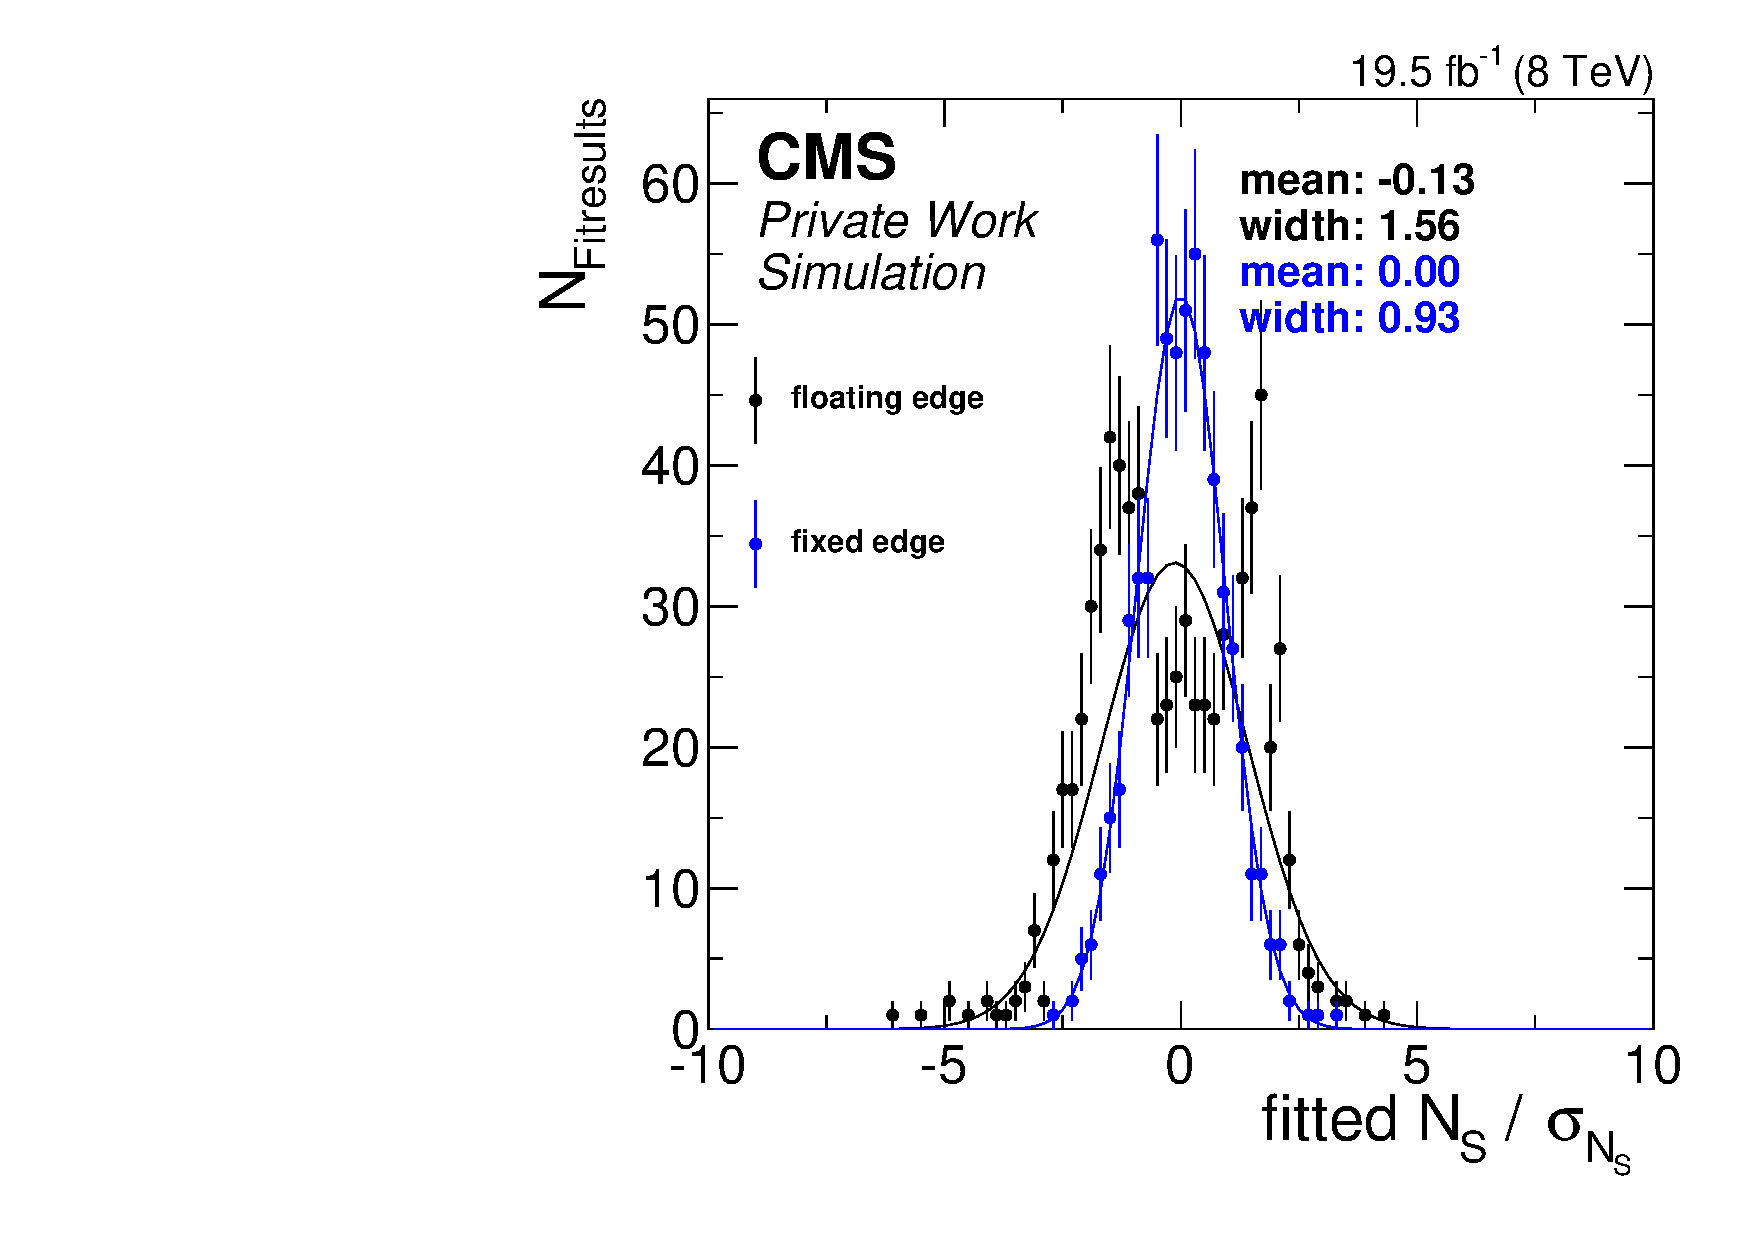
\includegraphics[width=\textwidth]{plots/results/fit/nS_floatVsFixed.pdf}
  \end{minipage}
  \begin{minipage}[t]{0.49\textwidth}
    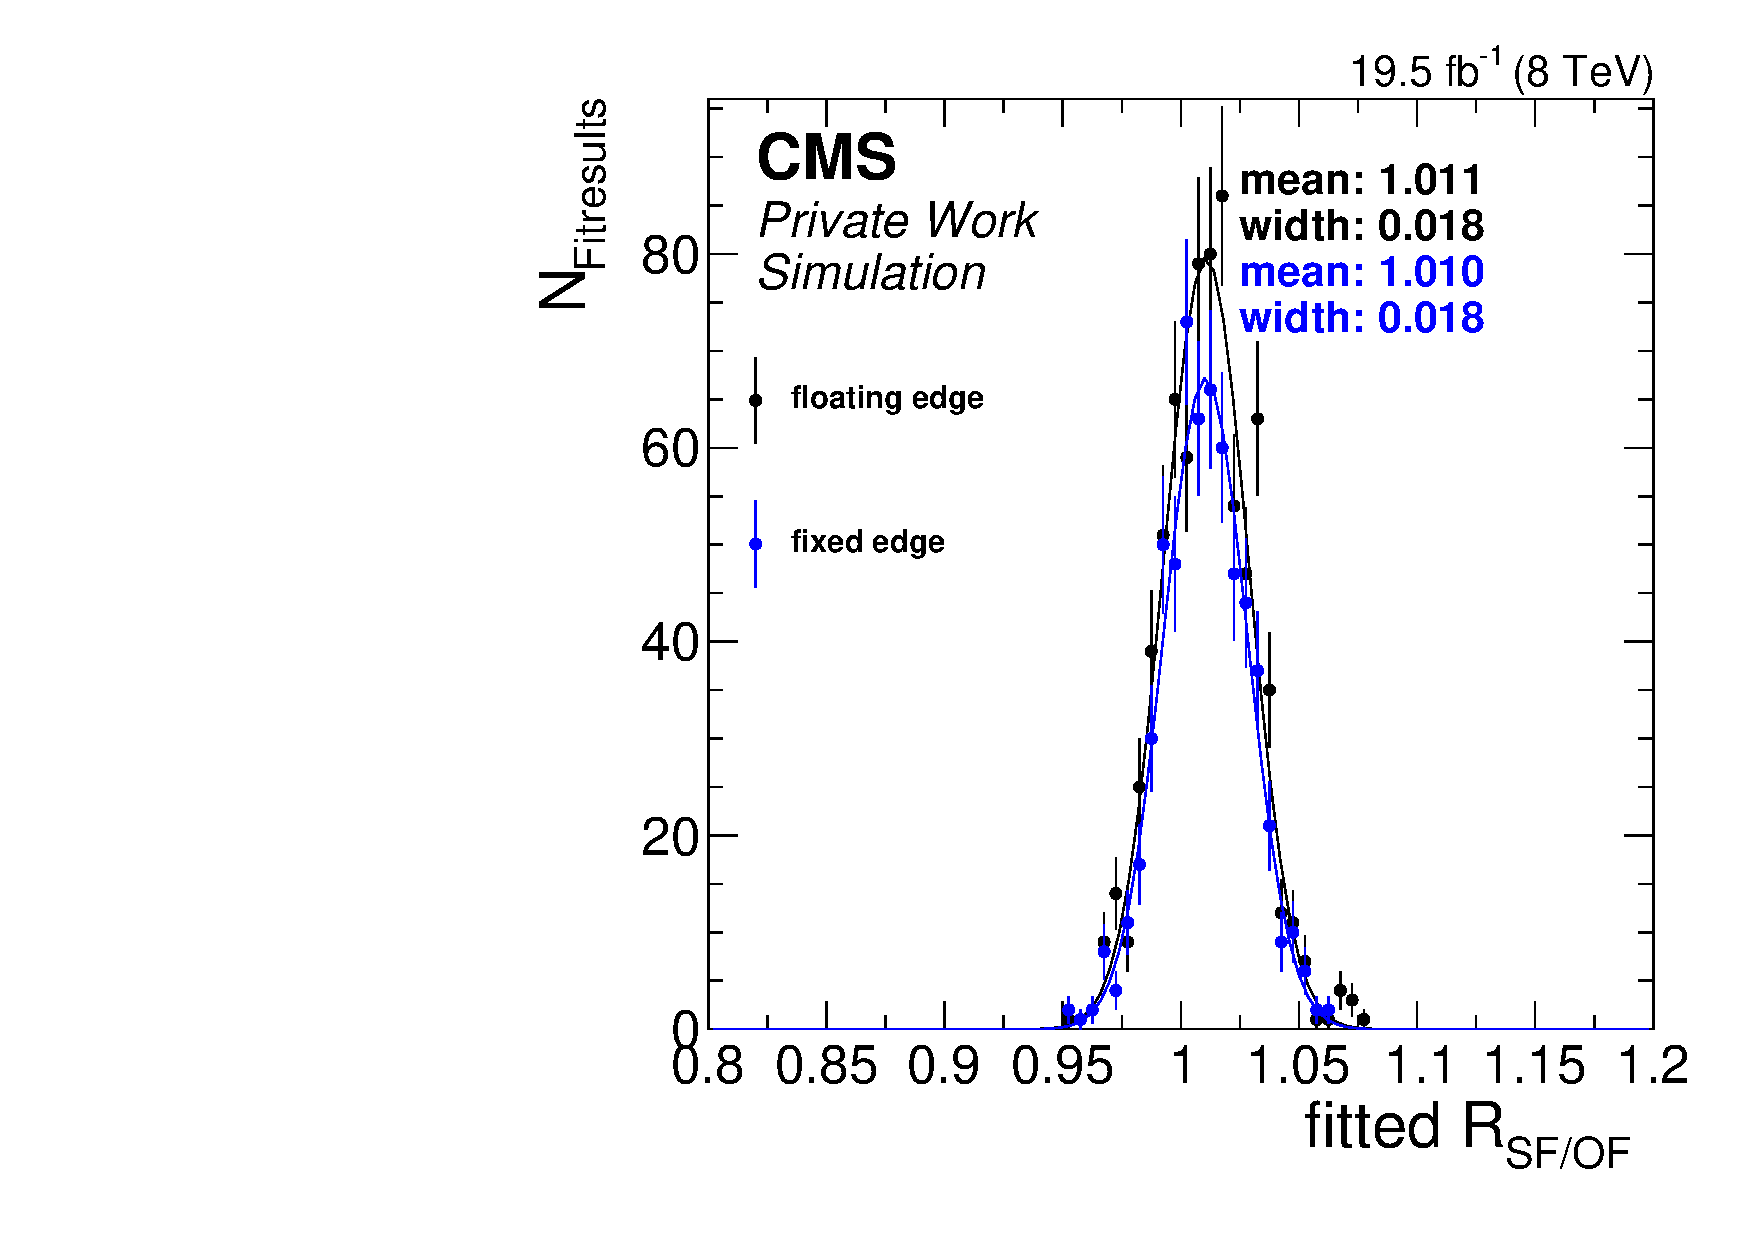
\includegraphics[width=\textwidth]{plots/results/fit/rSFOF_floatVsFixed.pdf}
  \end{minipage}

  \caption{Distribution of fit observables in toy studies for a background only scenario. Shown are the fitted number of signal events divided by their uncertainty in the central region (left) and the corresponding fitted values of \Rsfof (right). Shown are results for a floating edge (black) and a fixed edge position (blue).}
  \label{fig:toys:backgroundOnly}
\end{figure}

As an additional check, toys are generated with \Rsfof shifted by $\pm1\sigma$. These toys are fitted with the Gaussian constraint to the central value and the results are shown in Figure~\ref{fig:toys:systShift}. The same distributions are shown as above. In the case of the signal yield divided by its uncertainty, the double peak structure observed in the nominal configuration changes to a single peak that is shifted to negative signal yields for the toys generated with lower and to positive signal yields for those generated with higher values of \Rsfof. For the fitted values of \Rsfof, the width of the distribution is unchanged, but the systematic shifts in the generation of the toys is reflected in their means. However, the observed shifts of the mean (0.025 and -0.023) are smaller than those introduced the generation of the toys ($\pm0.037$, the uncertainty of \Rsfof), suggesting that part of the systematic shift is absorbed by the fit by introducing a signal contribution.
\begin{figure}[hbp]
  \centering
  \begin{minipage}[t]{0.49\textwidth}
    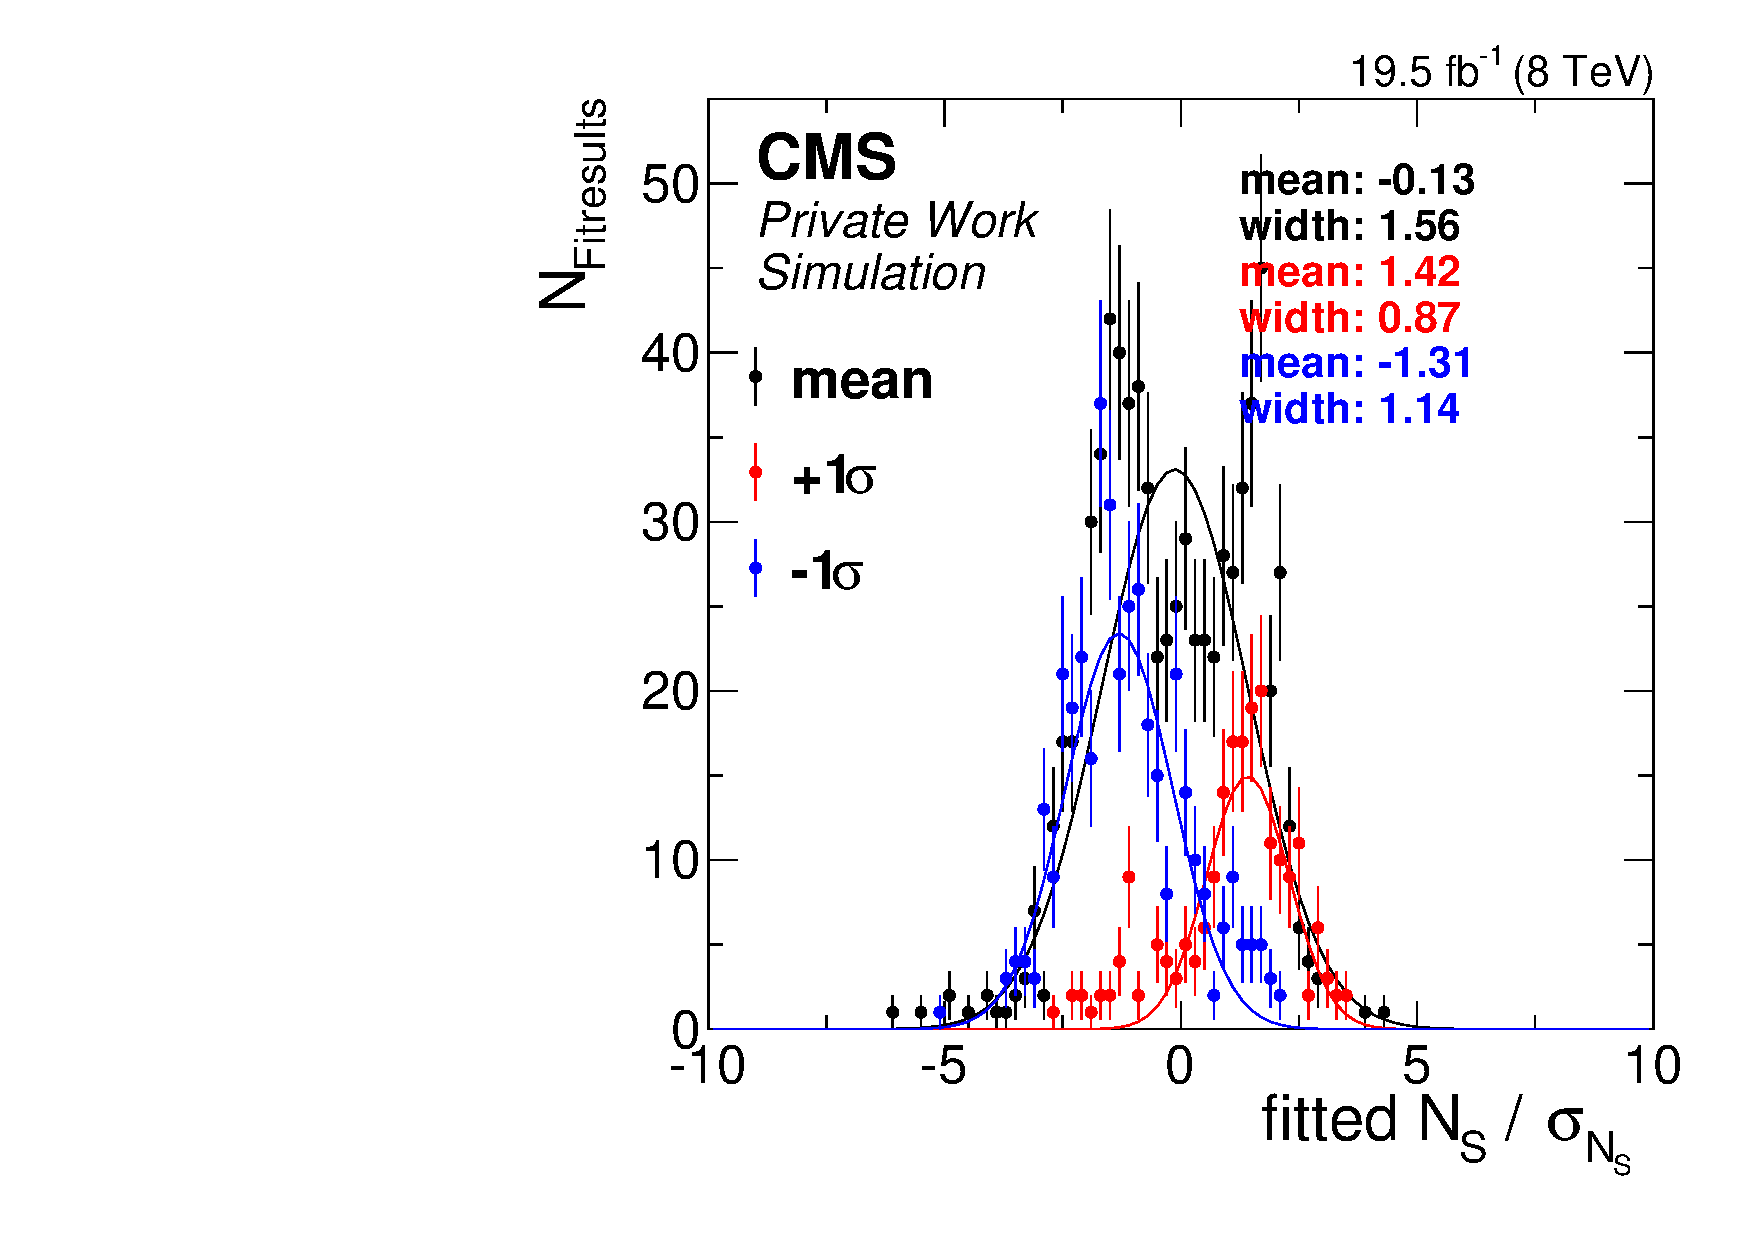
\includegraphics[width=\textwidth]{plots/results/fit/nS_systShift.pdf}
  \end{minipage}
  \begin{minipage}[t]{0.49\textwidth}
    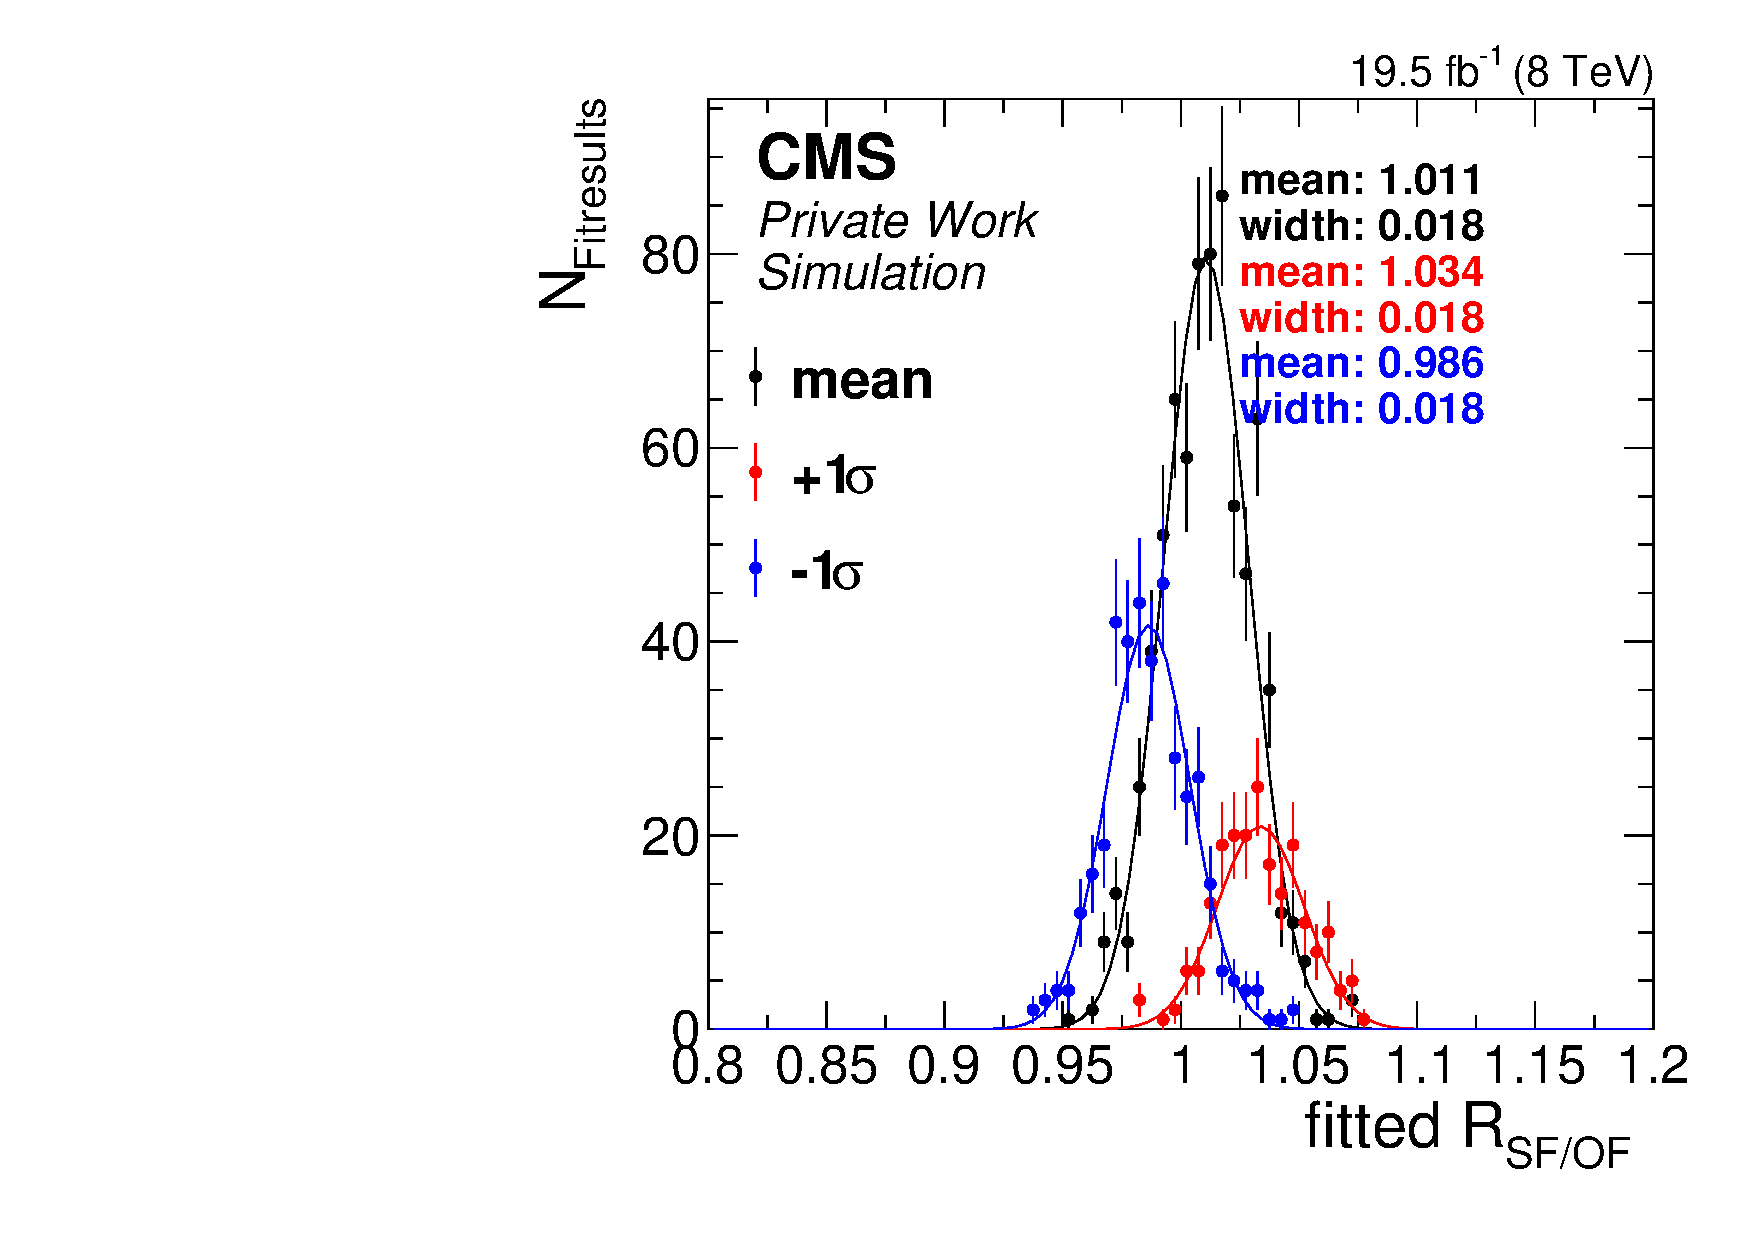
\includegraphics[width=\textwidth]{plots/results/fit/rSFOF_systShift.pdf}
  \end{minipage}

  \caption{Distribution of fit observables in toy studies for background only toys with fixed edge position. Shown are the fitted number of signal events in the central region (left) and the fitted number of signal events divided by the fitted uncertainty in the central region (right).}
  \label{fig:toys:systShift}
\end{figure}
\paragraph{Toy studies with signal injection}
The fit performance in the presence of a signal is tested by injection a signal of 125 events with and edge position of 70 GeV in the central region and again a third of that number in the forward signal region. Figure \ref{fig:toys:signalInjected} shows the resulting distribution of fit results for a selection of observables in the central signal region. The distribution of the number of signal events is well described by a Gaussian with a mean of about 126 events, very close to the injected number, and a width of 41 events. Divided by the fitted uncertainty this gives a unit Gaussian with a mean of about 2.9. The edge position is also Gaussian distributed, with a mean of about $\unit{70}{\giga\electronvolt}$, also reproducing the injected value very well, with a width of about $\unit{1.8}{\giga\electronvolt}$. Comparing the distribution of \Rsfof with that in Figure~\ref{fig:toys:backgroundOnly}, it can be seen that the presence of a signal does not bias the result towards higher values. 
\begin{figure}[hbp]
  \centering
  \begin{minipage}[t]{0.49\textwidth}
    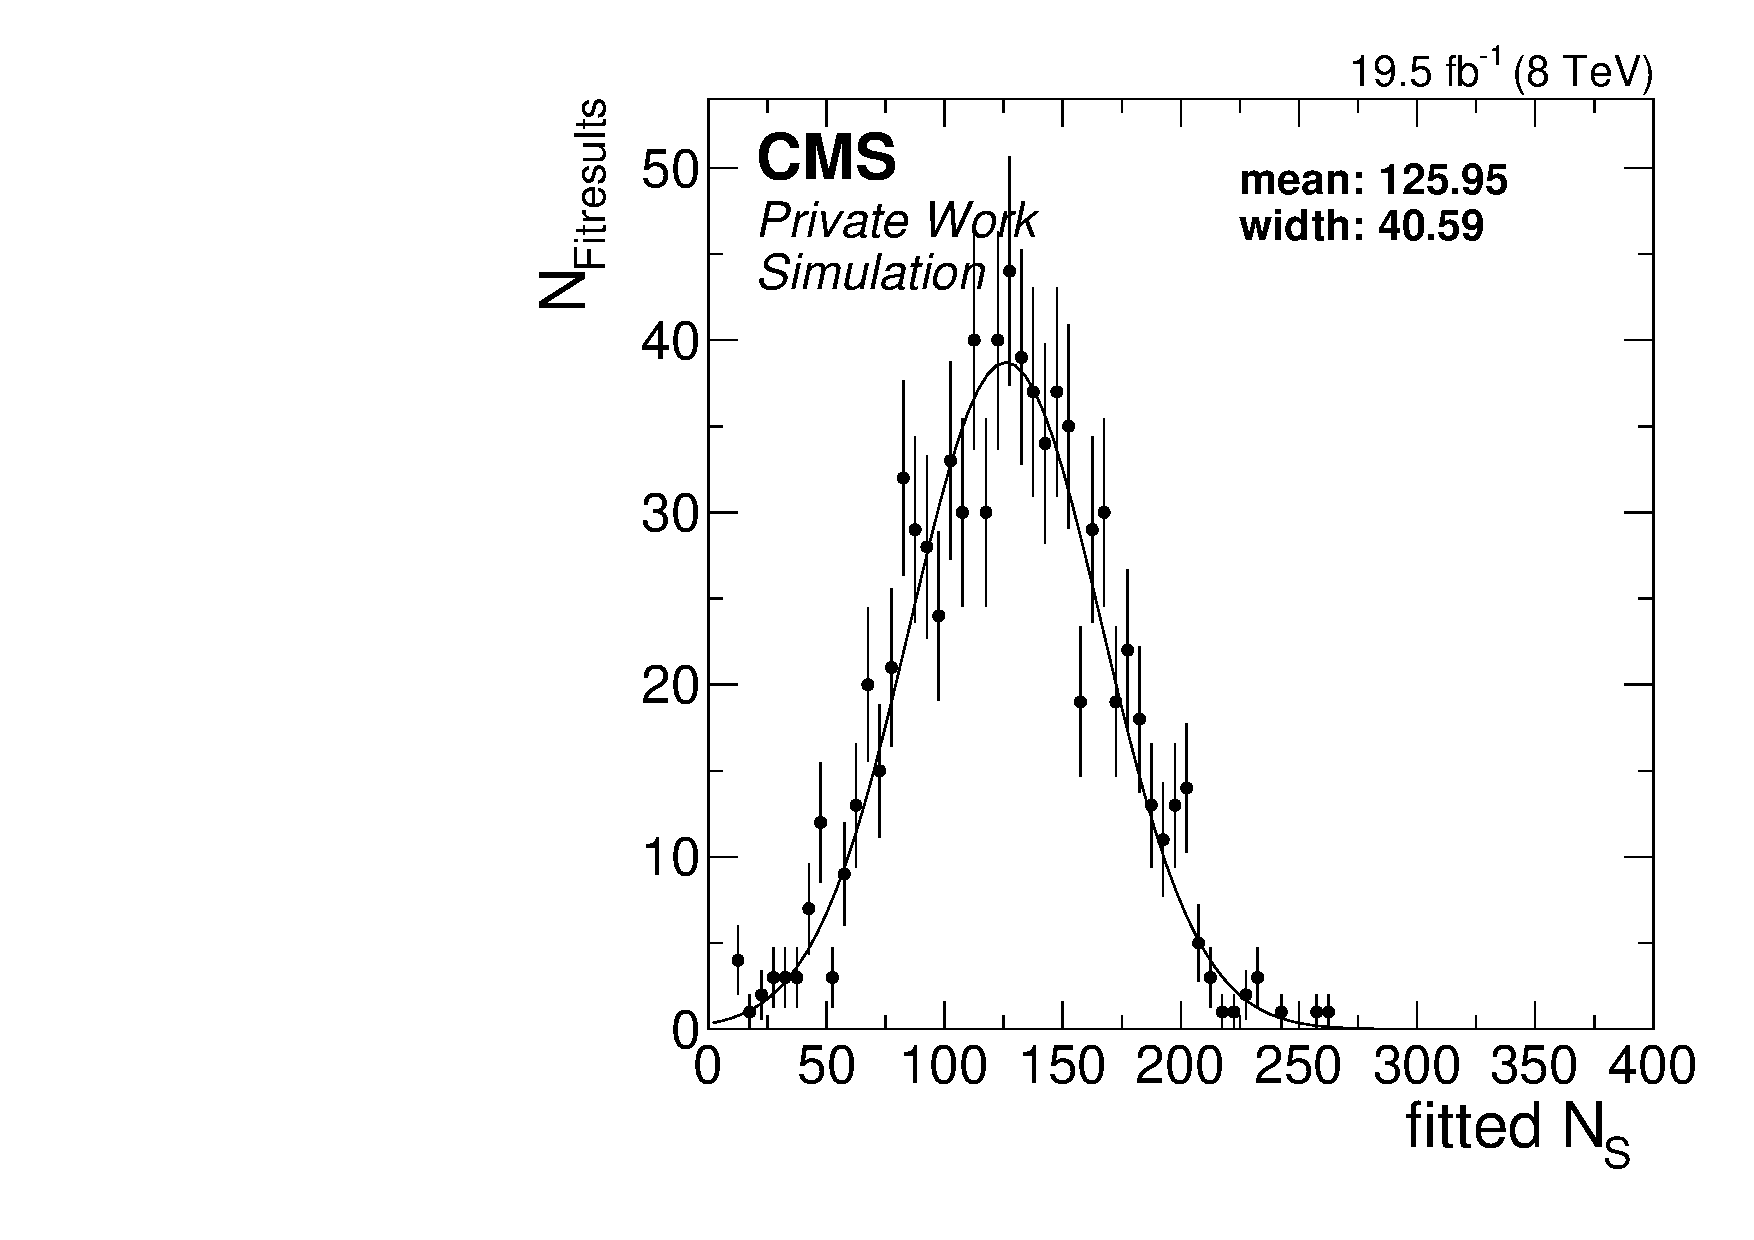
\includegraphics[width=\textwidth]{plots/results/fit/nSPure_signalInjected.pdf}
  \end{minipage}
  \begin{minipage}[t]{0.49\textwidth}
    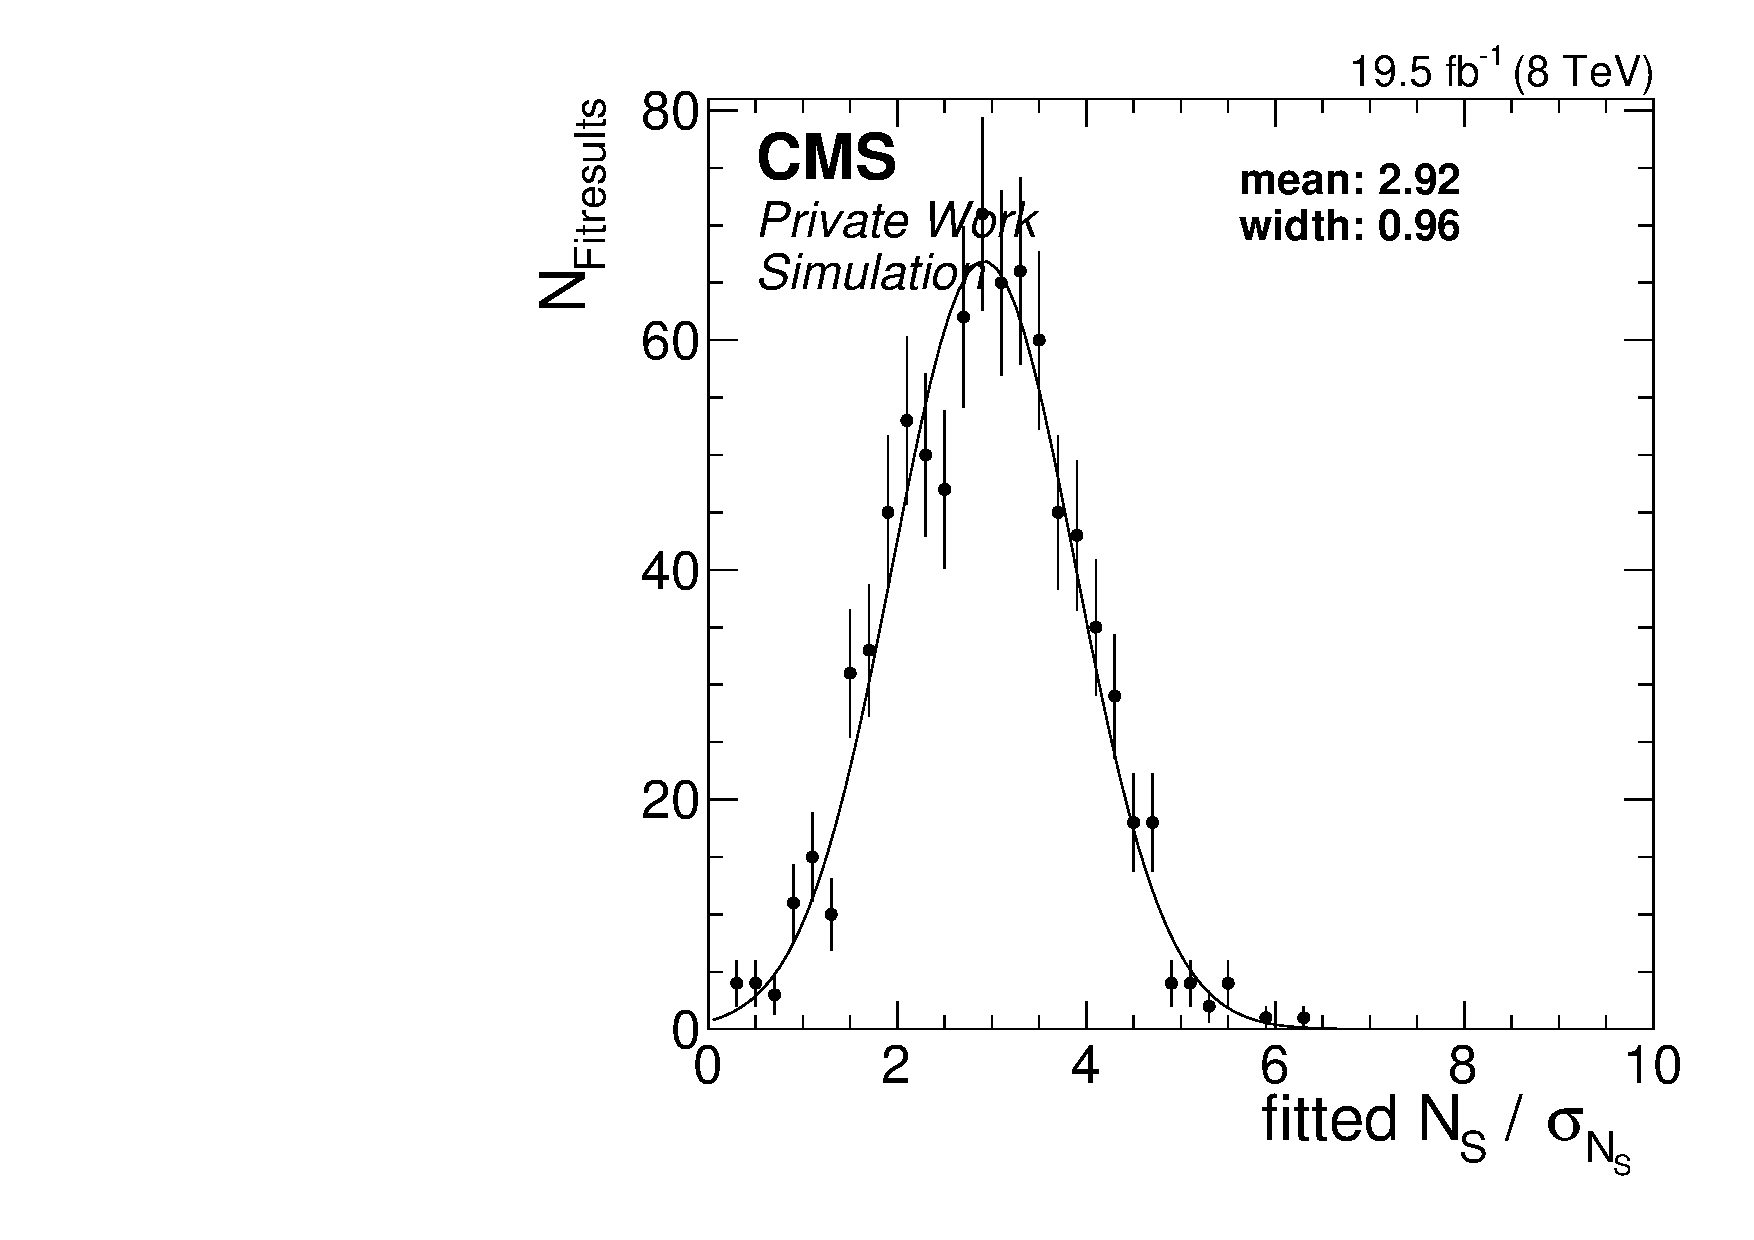
\includegraphics[width=\textwidth]{plots/results/fit/nS_signalInjected.pdf}
  \end{minipage}
  \begin{minipage}[t]{0.49\textwidth}
    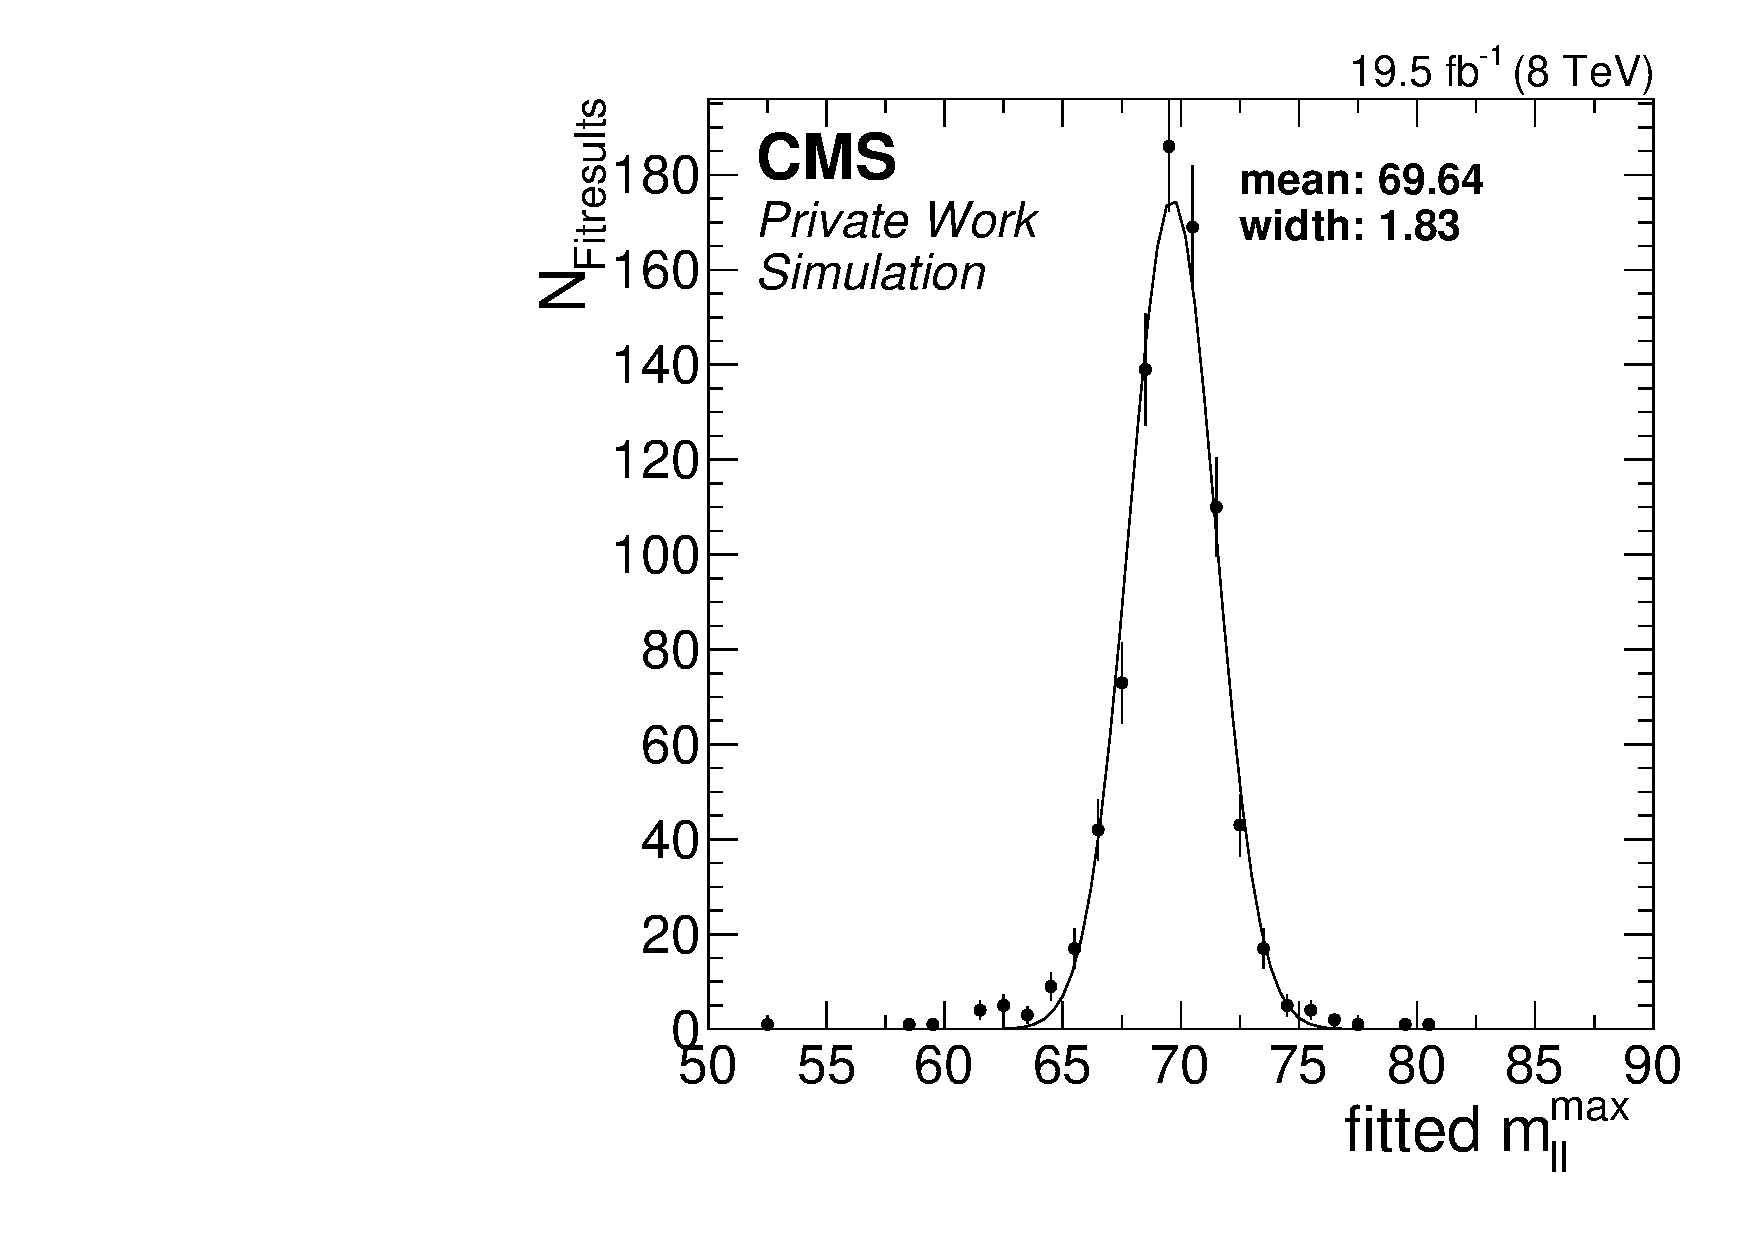
\includegraphics[width=\textwidth]{plots/results/fit/m0_signalInjected.pdf}
  \end{minipage}
  \begin{minipage}[t]{0.49\textwidth}
    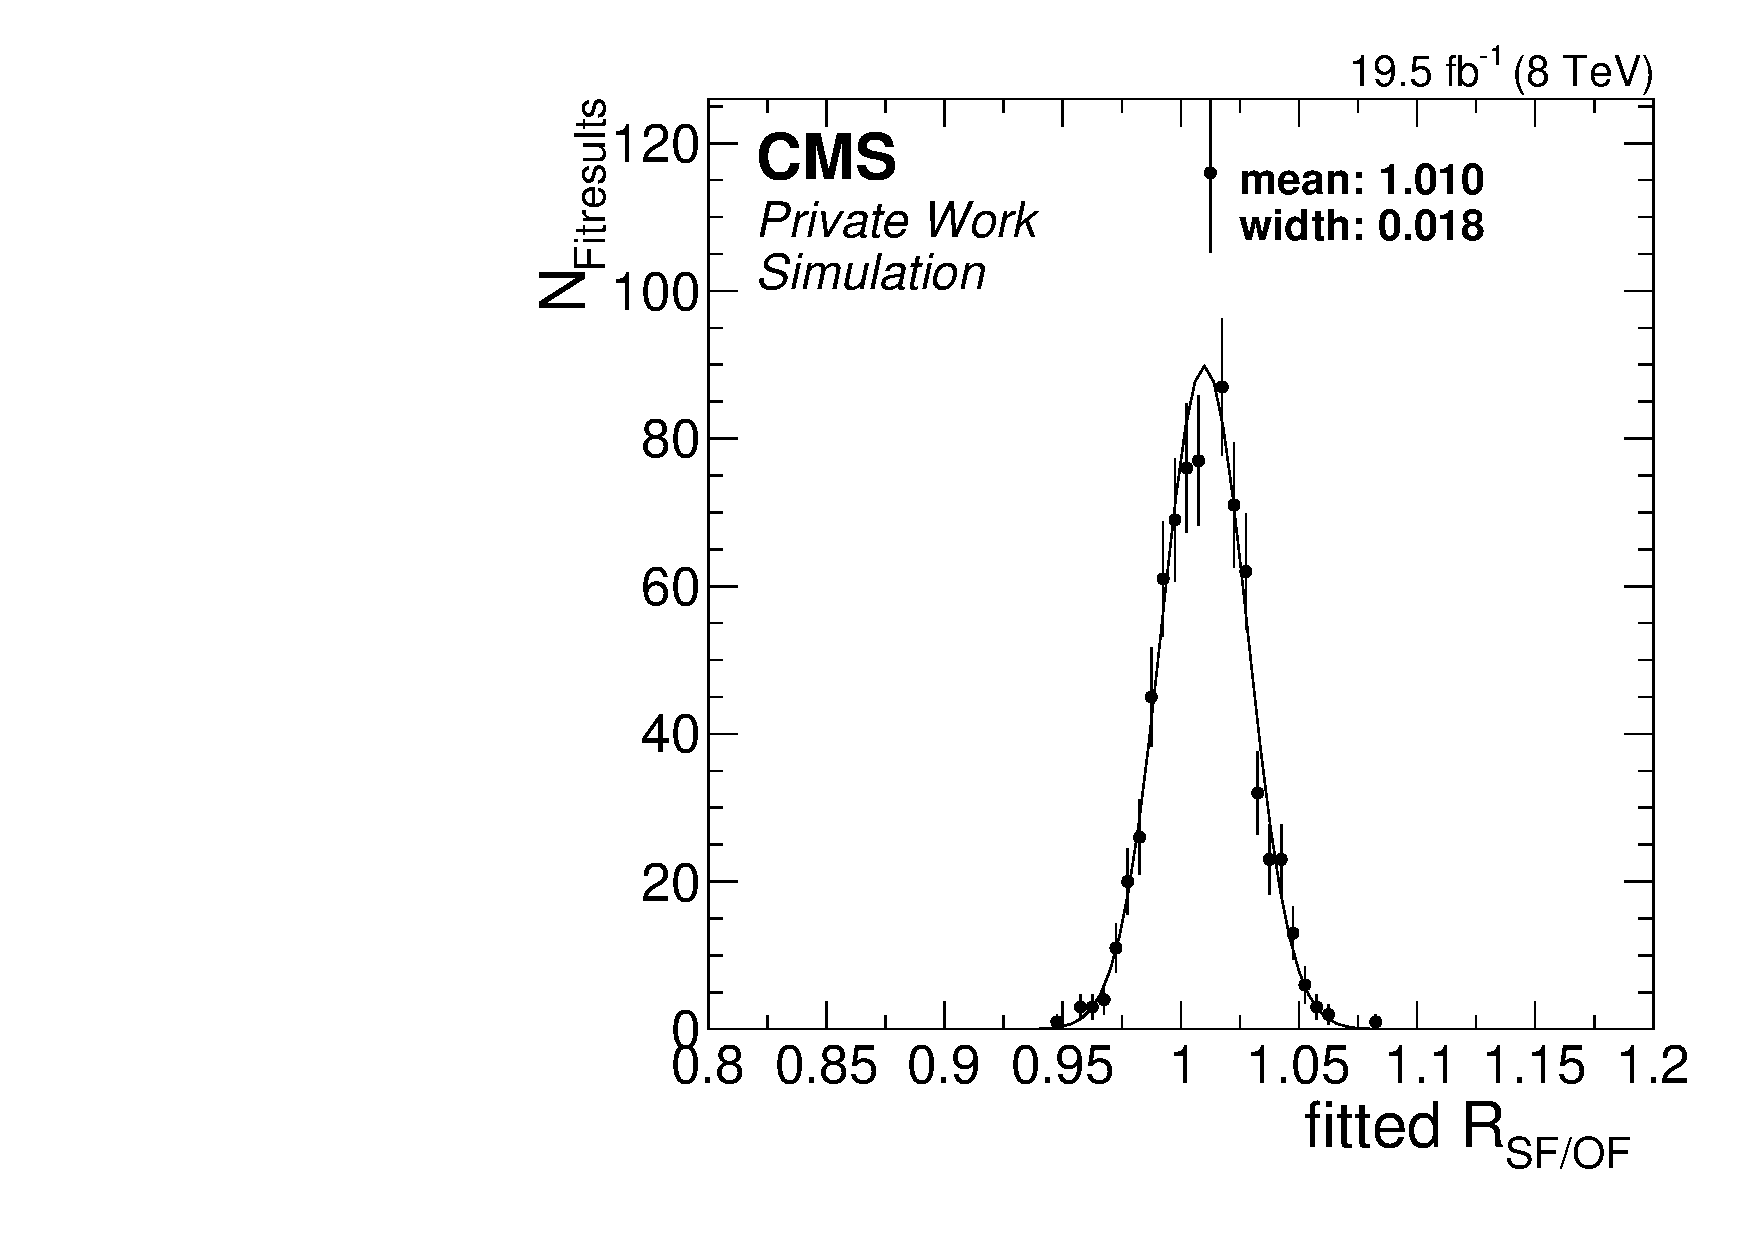
\includegraphics[width=\textwidth]{plots/results/fit/rSFOF_signalInjected.pdf}
  \end{minipage}
  \caption{Distribution of fit observables in toy studies with a signal injected. Shown are the fitted number of signal events in the central region (upper left), the fitted number of signal events divided by the fitted uncertainty in the central region (upper right), the fitted edge position (lower left) and the fitted \Rsfof in the central region (lower right).}
  \label{fig:toys:signalInjected}
\end{figure}
\newpage

\section{Results}
The result of the fit performed in the signal region on data is shown in Figure~\ref{fig:fit:result}. Shown are the \mll distributions in the SF and OF channels for the central and forward dilepton selection. The quantitative results are shown in Table~\ref{tab:fitResult}. Similar to the counting experiment, an excess of events is observed below the Z boson peak in the central signal region. The best fit value for the position of an edge is found to be $\unit{82.4}{\giga\electronvolt}$, with an signal yield of 140$\pm$47 events. No significant contribution of a signal is found in the forward region, where the fitted signal yield is 1$\pm$?? events. In the central region the fitted value of \Rsfof is slightly larger than the initial value, indicating that the fit absorbs some fraction of the excess into the background prediction. However, the difference is small compared to the fitted uncertainty and the uncertainty on the predicted value. In the forward region, the fitted value is smaller than the initial value, but also this deviation is well within the uncertainties. 


\begin{figure}[hbp]
  \centering
  \begin{minipage}[t]{0.49\textwidth}
    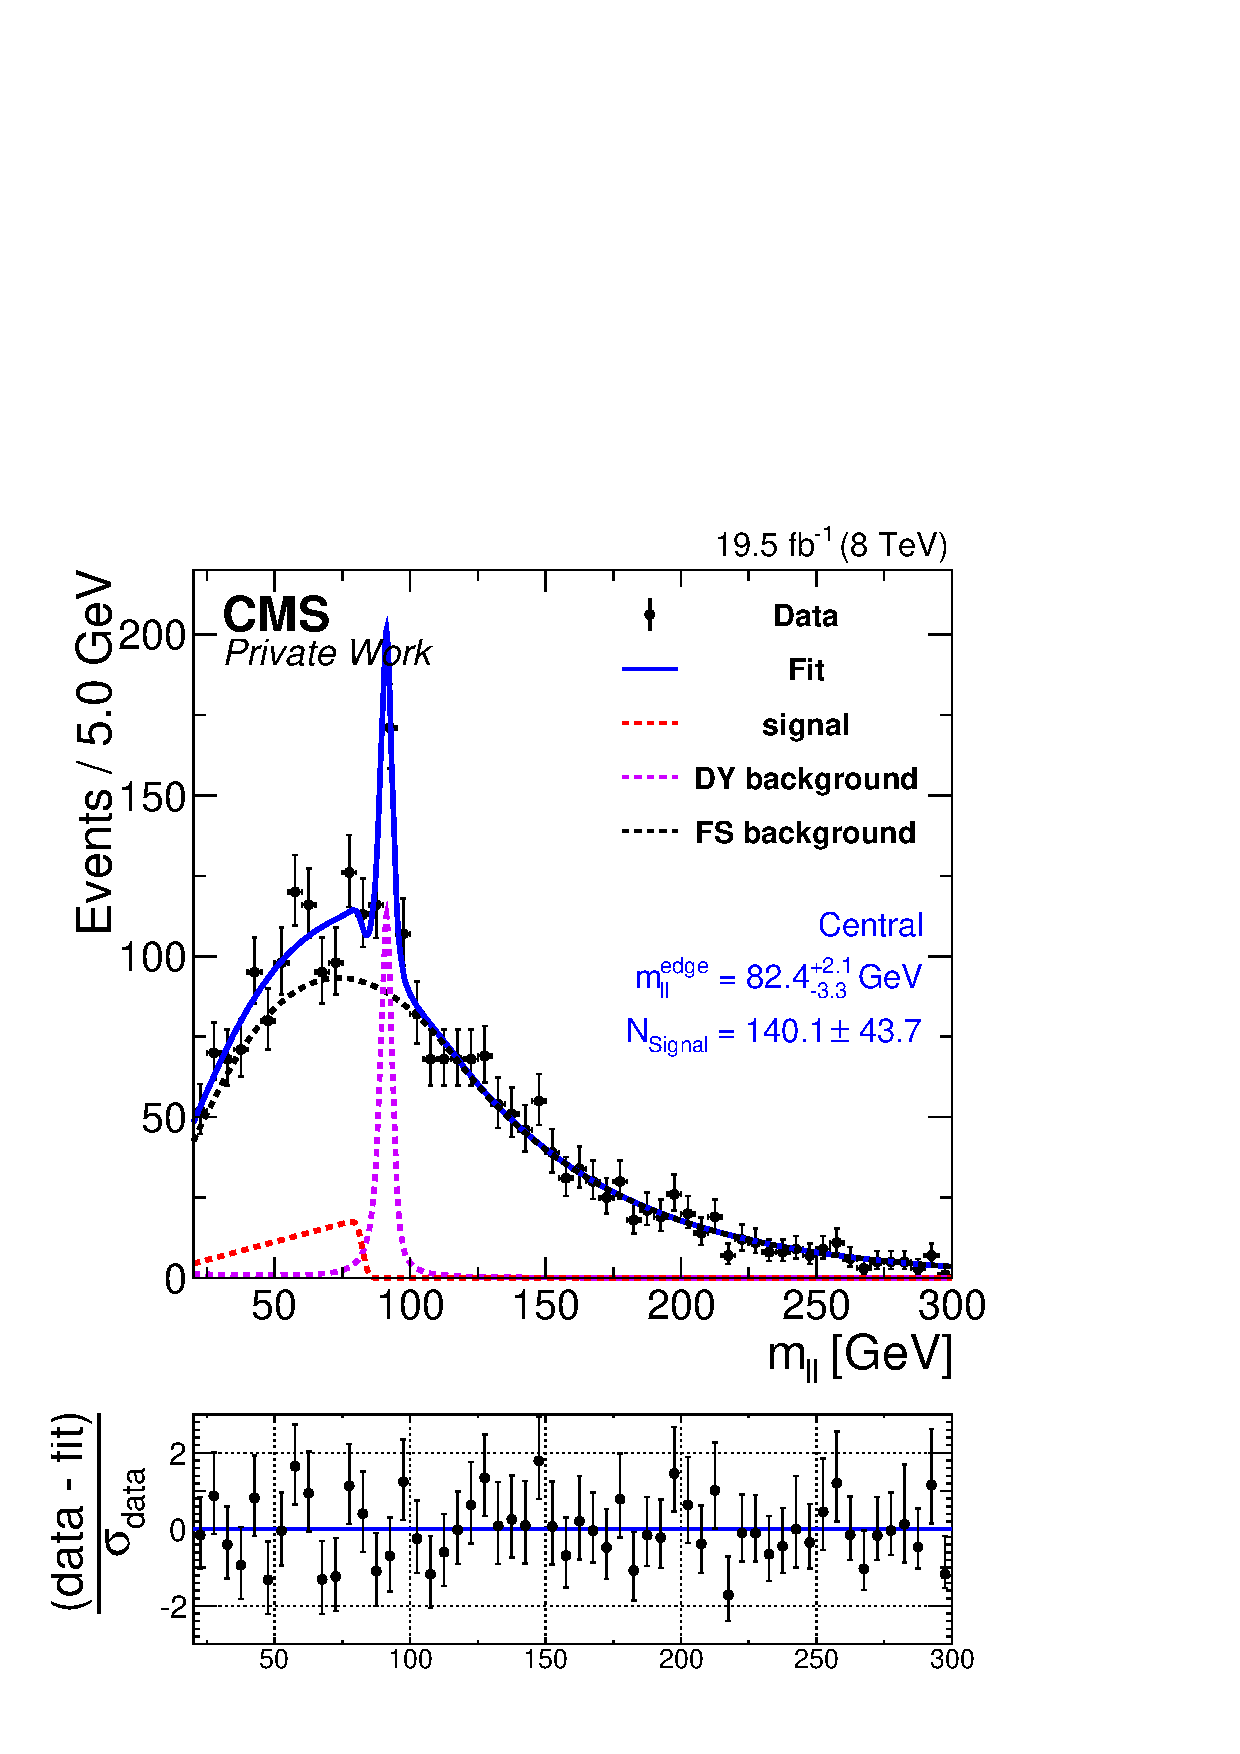
\includegraphics[width=\textwidth]{plots/results/fit/fit2012_ETHTriangle_SignalInclusive_Combined_Full2012_ETHTriangle_Central.pdf}
  \end{minipage}
  \begin{minipage}[t]{0.49\textwidth}
    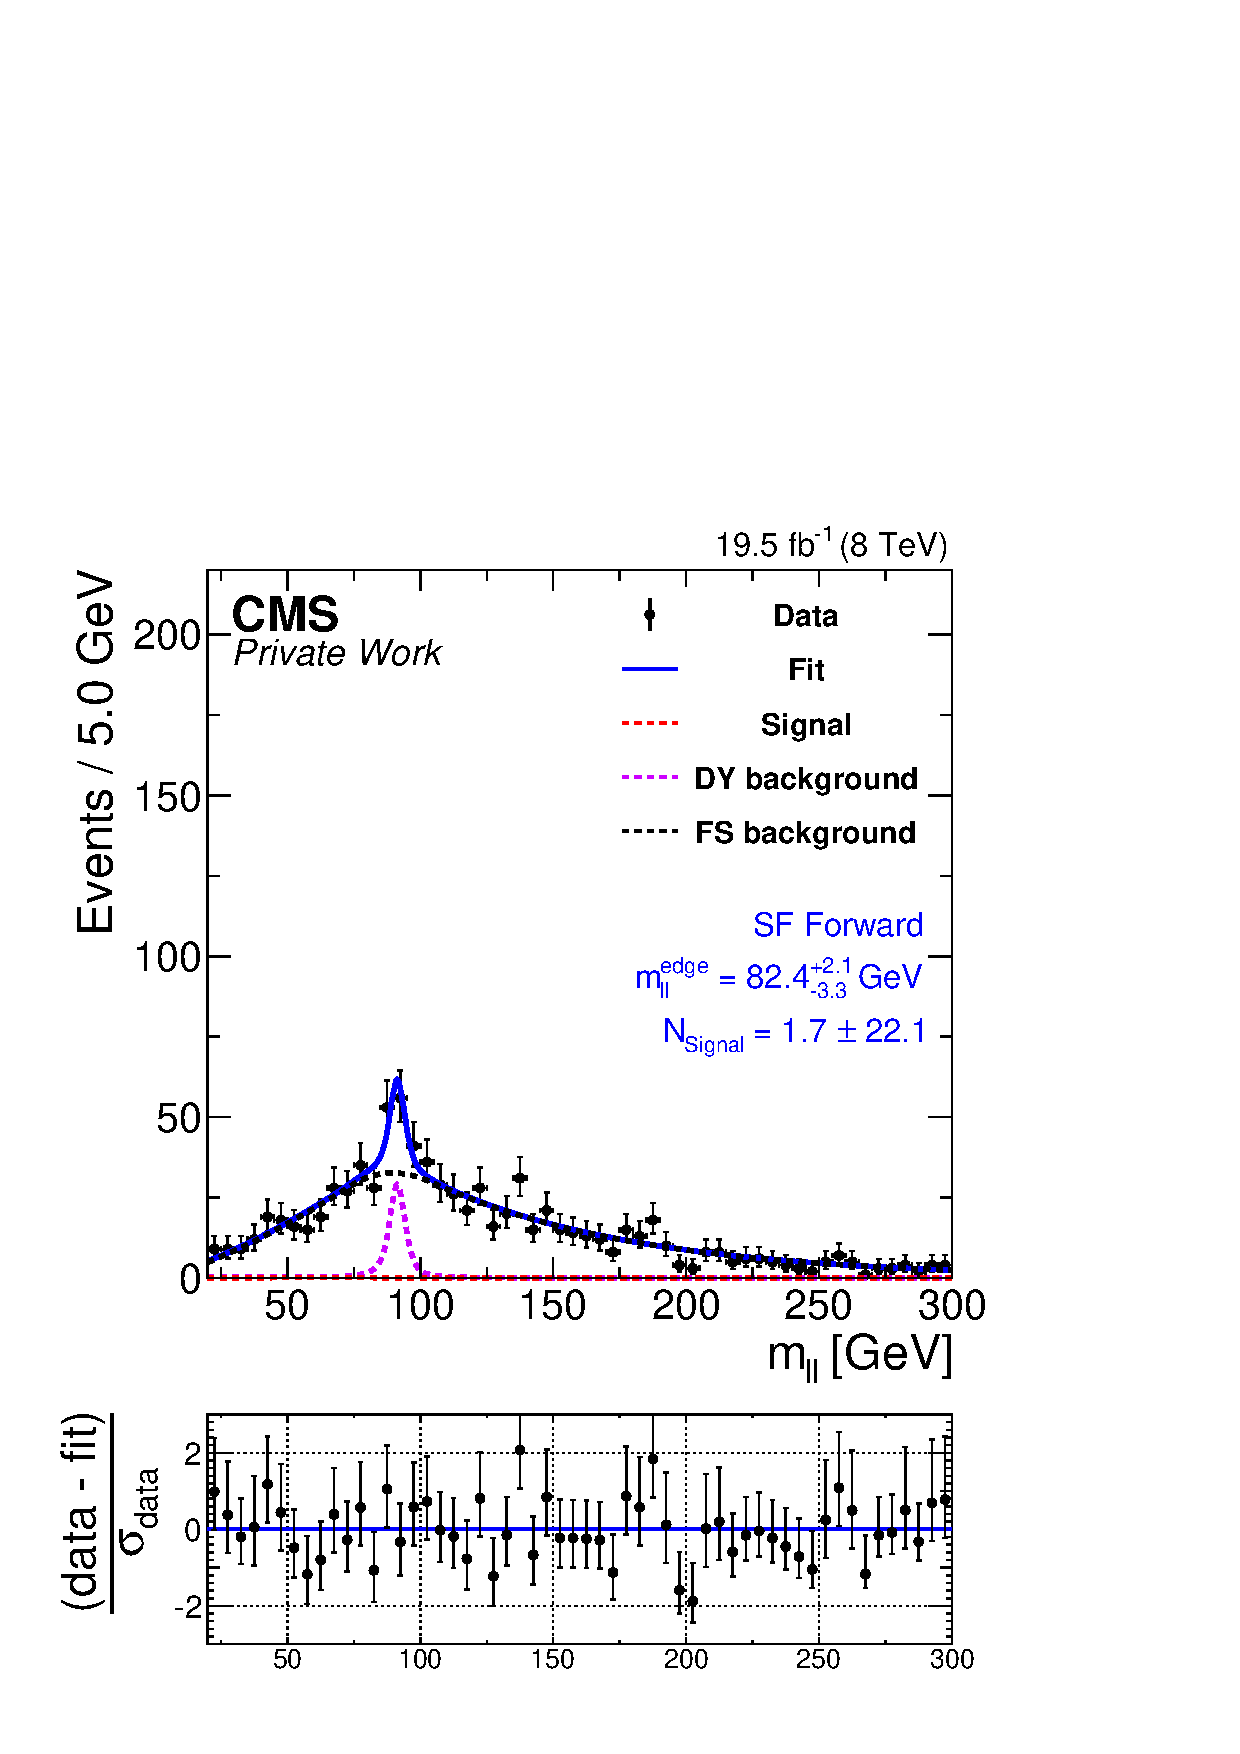
\includegraphics[width=\textwidth]{plots/results/fit/fit2012_ETHTriangle_SignalInclusive_Combined_Full2012_ETHTriangle_Forward.pdf}
  \end{minipage}
  \begin{minipage}[t]{0.49\textwidth}
    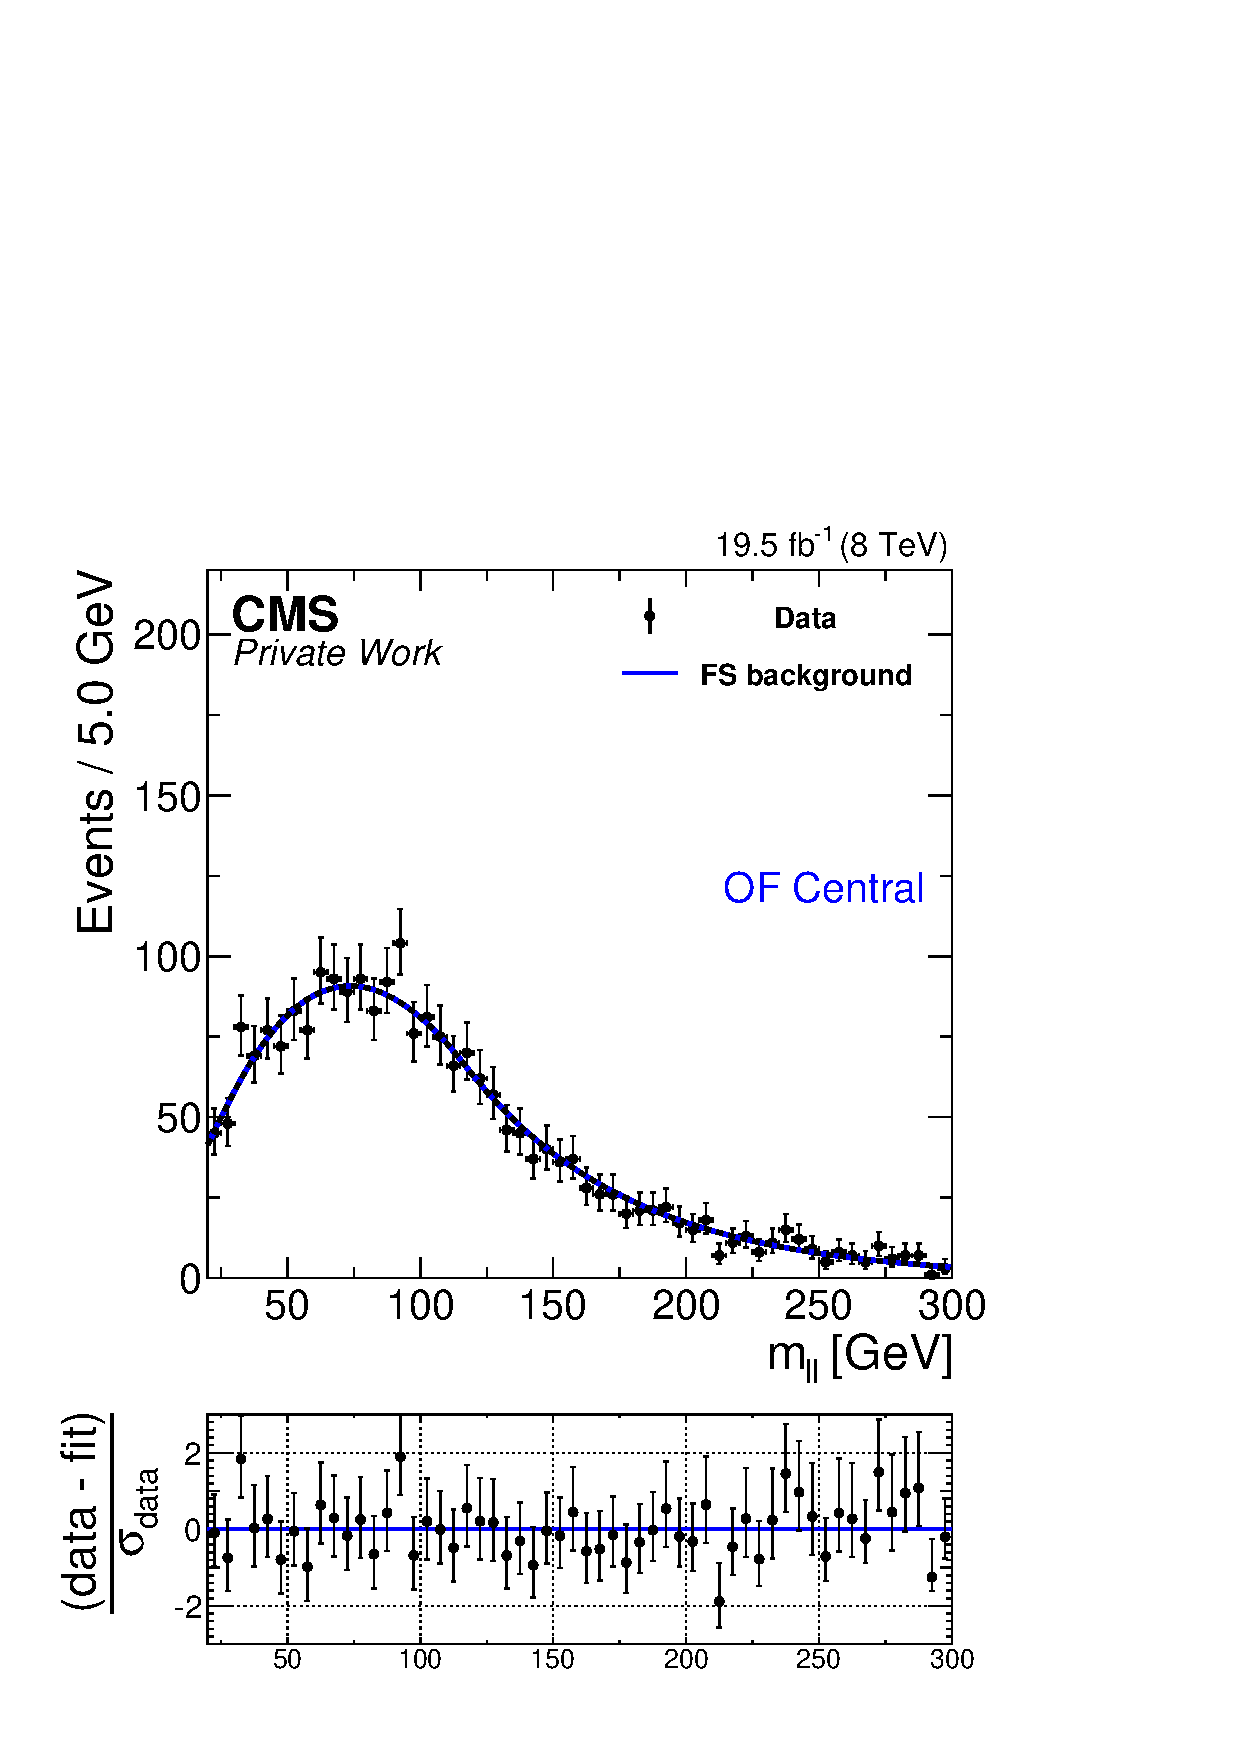
\includegraphics[width=\textwidth]{plots/results/fit/fit2012OFOS_ETHTriangle_SignalInclusive_Combined_Full2012_ETHTriangle_Central.pdf}
  \end{minipage}
  \begin{minipage}[t]{0.49\textwidth}
    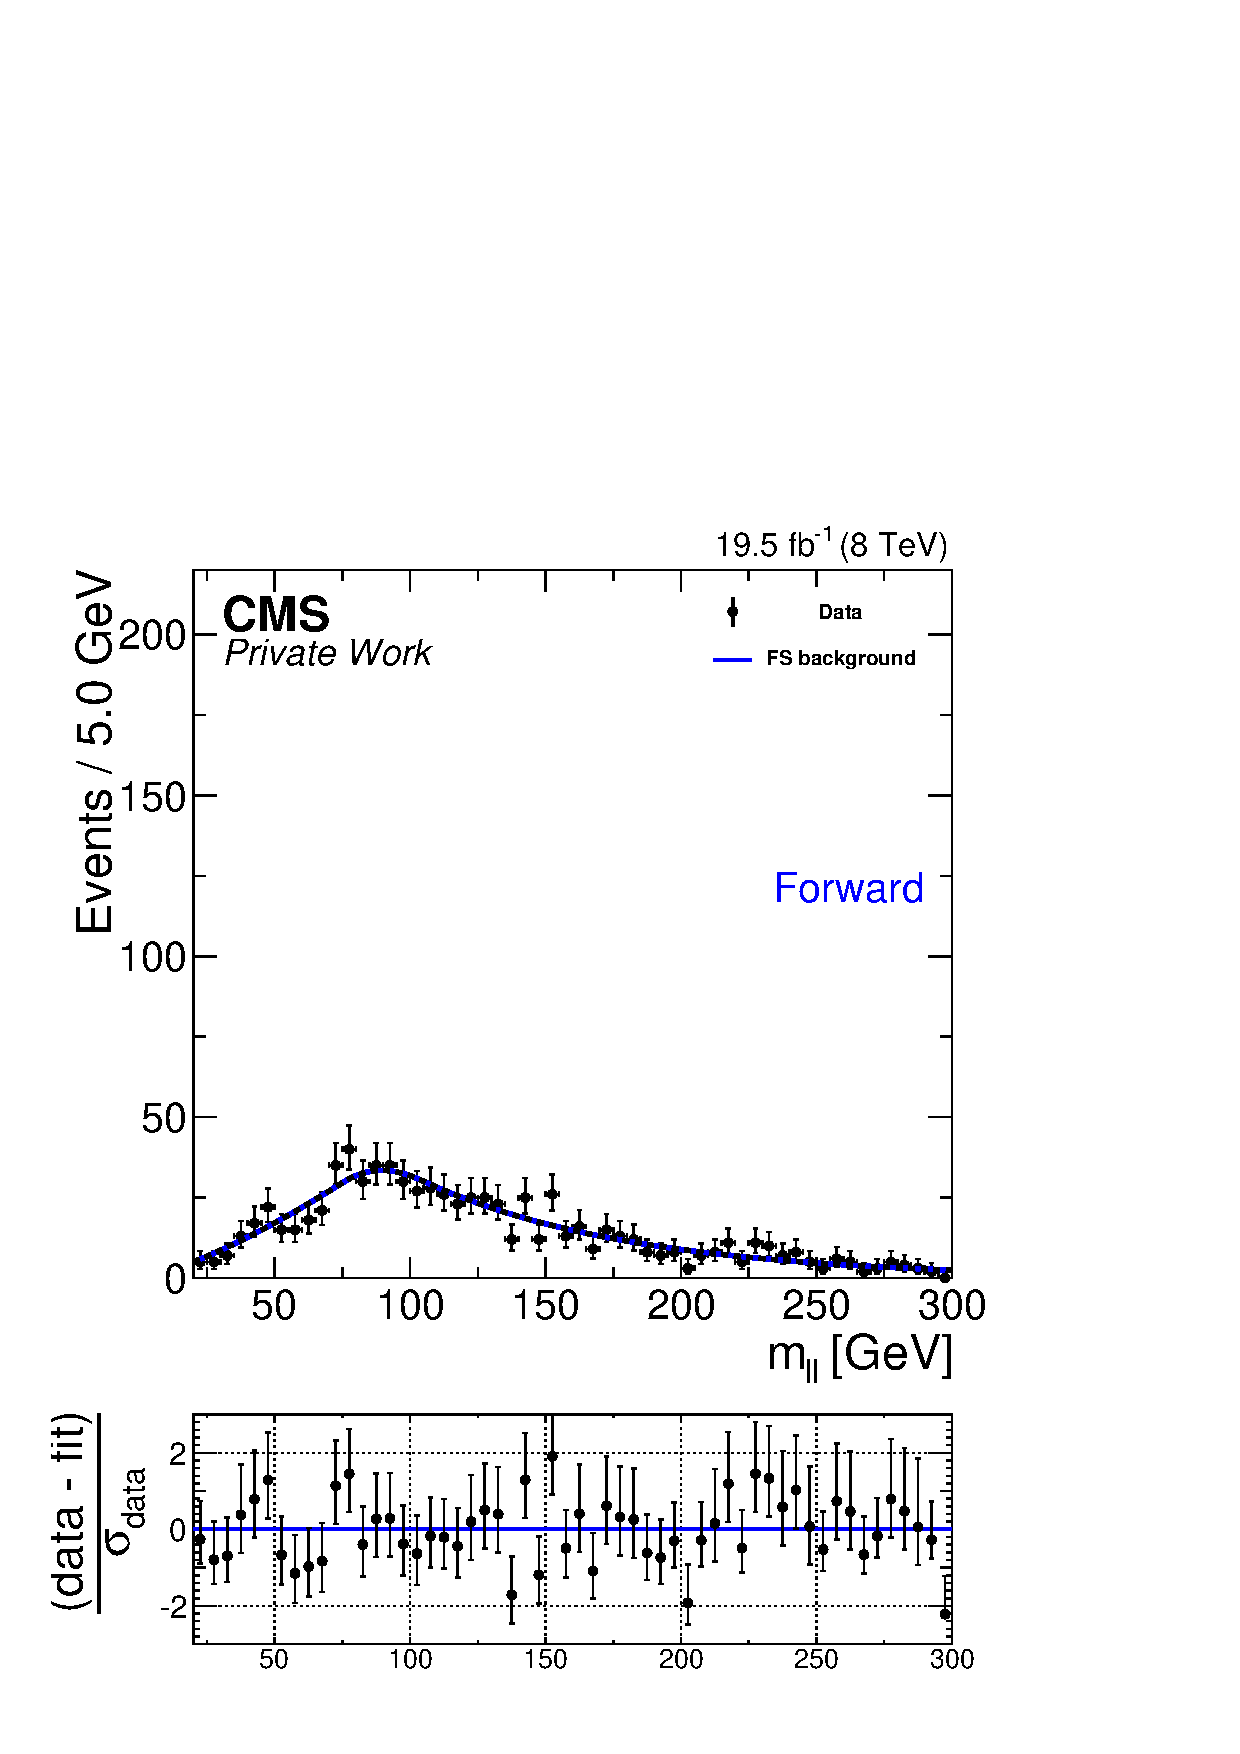
\includegraphics[width=\textwidth]{plots/results/fit/fit2012OFOS_ETHTriangle_SignalInclusive_Combined_Full2012_ETHTriangle_Forward.pdf}
  \end{minipage}
  \caption{Fit results in the signal region. Shown are the \mll distributions in SF (top) and OF (bottom) events for the central (right) and forward (left) dilepton selection. The fit is shown as a solid blue line while the different components are shown as dashed line, the signal model in red, the Drell--Yan model in violet and the flavour-symmetric model in black.}
  \label{fig:fit:result}
\end{figure}


\begin{table}[hbtp]
 \renewcommand{\arraystretch}{1.3}
 \setlength{\belowcaptionskip}{6pt}
 \centering
 \caption{Results of the fit in search for a kinematic edge in the signal region.
     }
  \label{tab:fitResult}
  \begin{tabular}{l| cc }
    \hline
    \hline
                                &  Central        & Forward \\ 

    \hline
        Drell--Yan background       &  170$\pm$23                   & 55$\pm$15  \\
        Flav. Sym. background in OF       &  2293$\pm$45                   & 792$\pm$25  \\
        \Rsfof       &  1.024$\pm$0.027                   & 1.012$\pm$0.042  \\
        signal events       &  140$\pm$44                   & 2$\pm$22  \\
        $m_{\ell\ell}^{edge}$ [GeV]       &  \multicolumn{2}{c}{$82.4^{+2.1}_{-3.3}$}  \\

\hline
\        local significance [$\sigma$]       &  \multicolumn{2}{c}{2.5 }  \\

    \hline
    \hline    
  \end{tabular}
\end{table}




A scan of the log-likelihood as a function of the edge position $m_{\ell\ell}^{egde}$ is shown in Figure~\ref{fig:fit:likelihoodScan}. The values have been shifted to set the minimum to zero. The curve exhibits a sharp drop at the best fit value for $m_{\ell\ell}^{egde}$, which is indeed the global minimum over the considered mass range. 

\begin{figure}[htbp]
\centering
  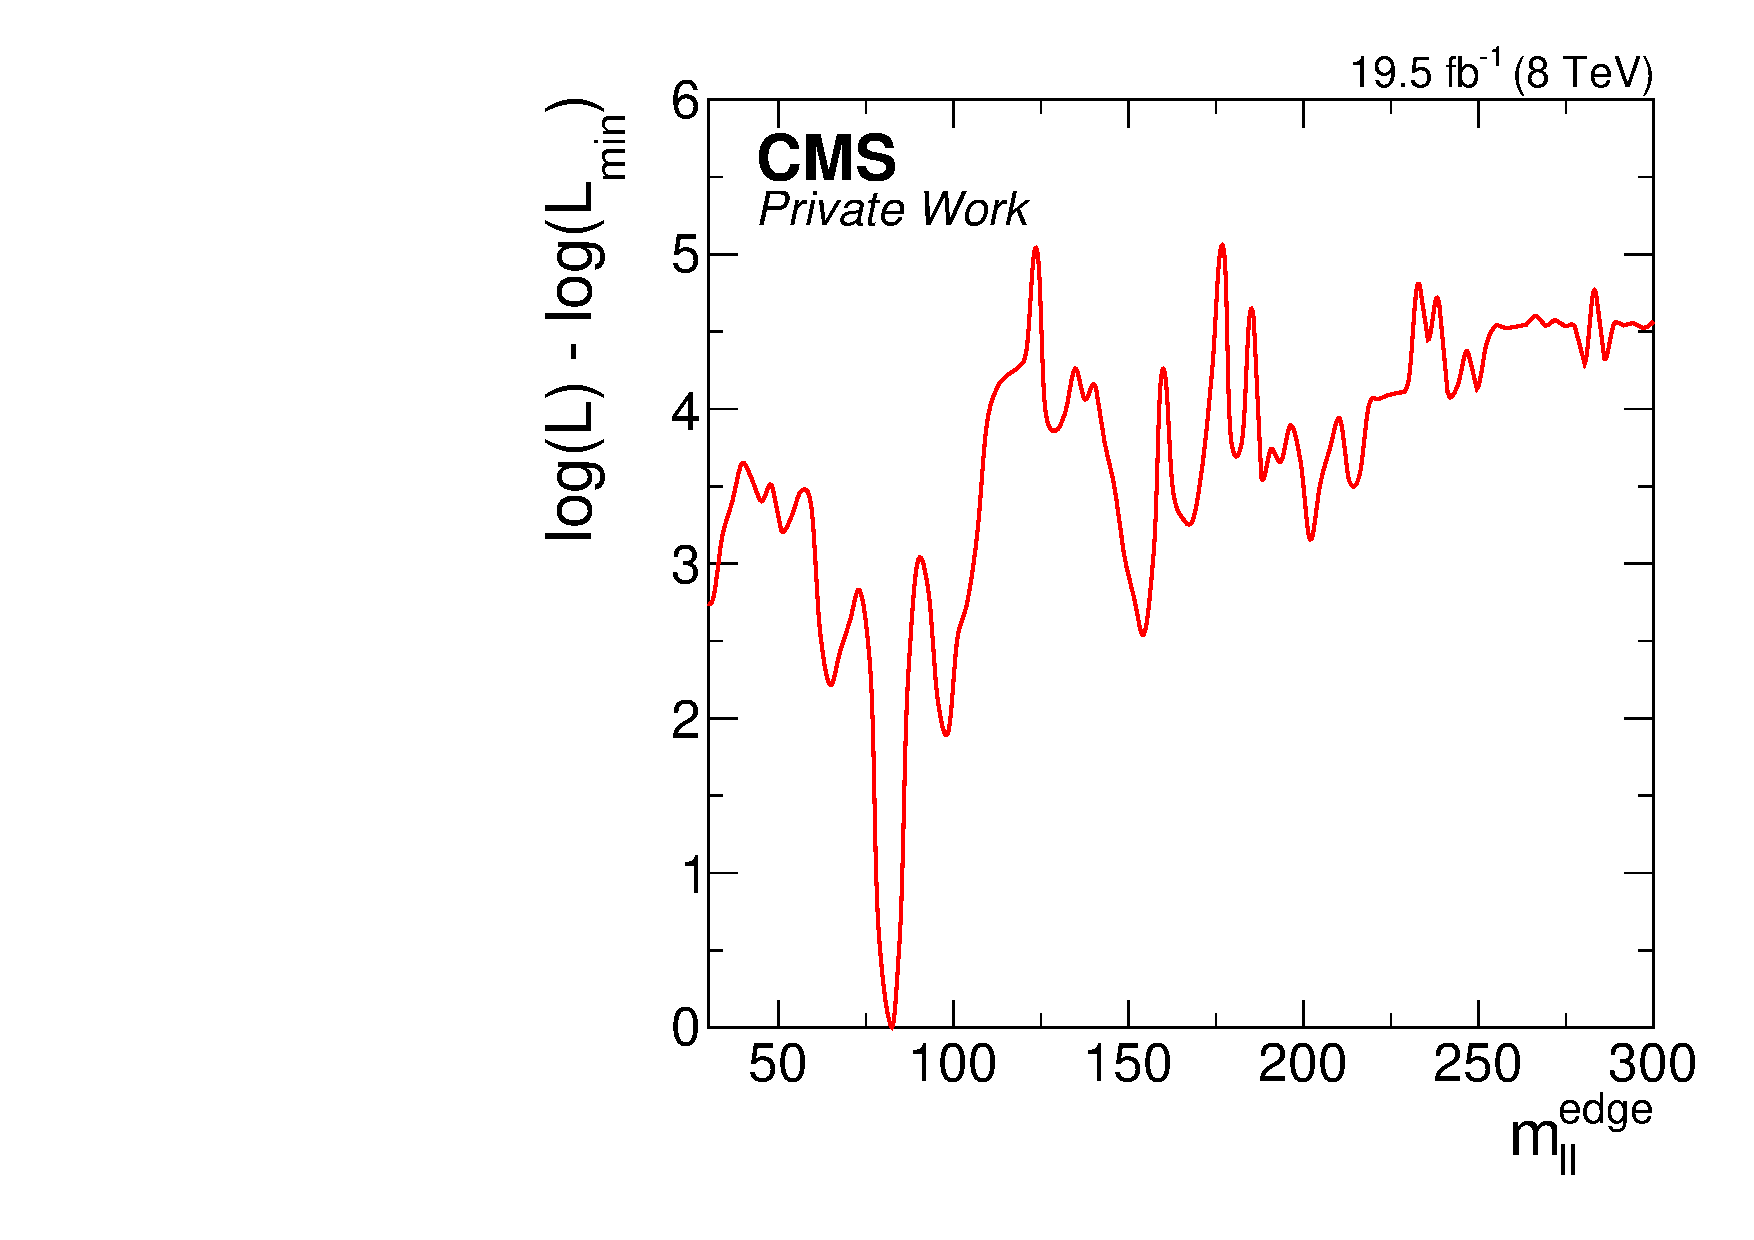
\includegraphics[width=0.6\textwidth]{plots/results/fit/signal.pdf}
\caption{Scan of the observed log-likelihood in the signal region subtracted by the minimal value as a function of $m_{\ell\ell}^{max}$.}
\label{fig:fit:likelihoodScan}
\end{figure}

As further validation of the result on data, the results obtained with different parametrization of the flavour-symmetric background are compared to the nominal result in Table~\ref{tab:fitComparison}. For the sake of clarity, only yields in the central signal region are shown. However, similar agreement is observed also in the forward signal region. In general, there is good agreement between all considered parametrizations. The best agreement is seen in the number of fitted flavour-symmetric events in the OF sample, which is expected as here the fit is mist simple, consisting only of one the shape for flavour-symmetric backgrounds. Good agreement is also observed for $m_{\ell\ell}^{egde}$ and the number of signal events, which are stable against the choice of background model. The most differences are observed for \Rsfof and the yield of the Z model. Here the fit can trade one against the other, depending on the parametrization of the flavour-symmetric background. Here the largest deviations are observed for the shape used in the analysis of the $\unit{7}{\tera\electronvolt}$ dataset. As this shape is known to not satisfactorily described the flavour-symmetric background, it is encouraging to see that the fit result is stable against such biases. The observed local significance is very similar among all analytical parametrizations. In the case of the KDE and the binned parametrization, the shape of the distribution is not free in the fit, as discussed above, excluding the statistical uncertainty of the OF sample from the fit and resulting in an systematically larger local significance. 



\begin{table}[hbtp]
 \renewcommand{\arraystretch}{1.3}
 \setlength{\belowcaptionskip}{6pt}
 \centering
 \caption{Comparison of edge fit results in the signal region for different parametrizations of the flavour-symmetric background. Results are given for the central signal region only. Similar agreement between the parametrization is also observed in the forward signal region.
     }
  \label{tab:fitComparison}
  \begin{tabular}{l| c c c c c c }
    \hline
    \hline
                                &  $N_{DY}$  & $N_{FS}$ & \Rsfof & $N_{S}$ &  $m_{\ell\ell}^{edge}$ [GeV]  & local $\sigma$ \\ 

    \hline
        nominal       &  170$\pm$23  &  2293$\pm$45 &  1.024$\pm$0.027 &  140$\pm$43 &   $82.4^{+2.1}_{-3.3}$      & 2.5  \\
        sum of Gaussians       &  168$\pm$24  &  2292$\pm$44 &  1.023$\pm$0.027 &  146$\pm$50 &   $82.1^{+2.2}_{-3.7}$      & 2.7  \\
        kernel density estimation       &  154$\pm$22  &  2296$\pm$43 &  1.028$\pm$0.026 &  141$\pm$41 &   $81.7^{+2.3}_{-3.4}$      & 3.1  \\
        histogram       &  140$\pm$23  &  2296$\pm$43 &  1.029$\pm$0.026 &  153$\pm$41 &   $83.0^{+1.7}_{-2.4}$      & 3.5  \\
        2011 shape       &  181$\pm$23  &  2290$\pm$43 &  1.020$\pm$0.026 &  146$\pm$46 &   $82.8^{+1.9}_{-2.5}$      & 2.7  \\

    \hline
    \hline    
  \end{tabular}
\end{table}


